% Options for packages loaded elsewhere
\PassOptionsToPackage{unicode}{hyperref}
\PassOptionsToPackage{hyphens}{url}
%
\documentclass[
]{book}
\usepackage{amsmath,amssymb}
\usepackage{lmodern}
\usepackage{ifxetex,ifluatex}
\ifnum 0\ifxetex 1\fi\ifluatex 1\fi=0 % if pdftex
  \usepackage[T1]{fontenc}
  \usepackage[utf8]{inputenc}
  \usepackage{textcomp} % provide euro and other symbols
\else % if luatex or xetex
  \usepackage{unicode-math}
  \defaultfontfeatures{Scale=MatchLowercase}
  \defaultfontfeatures[\rmfamily]{Ligatures=TeX,Scale=1}
\fi
% Use upquote if available, for straight quotes in verbatim environments
\IfFileExists{upquote.sty}{\usepackage{upquote}}{}
\IfFileExists{microtype.sty}{% use microtype if available
  \usepackage[]{microtype}
  \UseMicrotypeSet[protrusion]{basicmath} % disable protrusion for tt fonts
}{}
\makeatletter
\@ifundefined{KOMAClassName}{% if non-KOMA class
  \IfFileExists{parskip.sty}{%
    \usepackage{parskip}
  }{% else
    \setlength{\parindent}{0pt}
    \setlength{\parskip}{6pt plus 2pt minus 1pt}}
}{% if KOMA class
  \KOMAoptions{parskip=half}}
\makeatother
\usepackage{xcolor}
\IfFileExists{xurl.sty}{\usepackage{xurl}}{} % add URL line breaks if available
\IfFileExists{bookmark.sty}{\usepackage{bookmark}}{\usepackage{hyperref}}
\hypersetup{
  pdftitle={Urejanje podatkov},
  pdfauthor={Gregor Pirš, Matej Pičulin in Erik Štrumbelj},
  hidelinks,
  pdfcreator={LaTeX via pandoc}}
\urlstyle{same} % disable monospaced font for URLs
\usepackage{color}
\usepackage{fancyvrb}
\newcommand{\VerbBar}{|}
\newcommand{\VERB}{\Verb[commandchars=\\\{\}]}
\DefineVerbatimEnvironment{Highlighting}{Verbatim}{commandchars=\\\{\}}
% Add ',fontsize=\small' for more characters per line
\usepackage{framed}
\definecolor{shadecolor}{RGB}{248,248,248}
\newenvironment{Shaded}{\begin{snugshade}}{\end{snugshade}}
\newcommand{\AlertTok}[1]{\textcolor[rgb]{0.94,0.16,0.16}{#1}}
\newcommand{\AnnotationTok}[1]{\textcolor[rgb]{0.56,0.35,0.01}{\textbf{\textit{#1}}}}
\newcommand{\AttributeTok}[1]{\textcolor[rgb]{0.77,0.63,0.00}{#1}}
\newcommand{\BaseNTok}[1]{\textcolor[rgb]{0.00,0.00,0.81}{#1}}
\newcommand{\BuiltInTok}[1]{#1}
\newcommand{\CharTok}[1]{\textcolor[rgb]{0.31,0.60,0.02}{#1}}
\newcommand{\CommentTok}[1]{\textcolor[rgb]{0.56,0.35,0.01}{\textit{#1}}}
\newcommand{\CommentVarTok}[1]{\textcolor[rgb]{0.56,0.35,0.01}{\textbf{\textit{#1}}}}
\newcommand{\ConstantTok}[1]{\textcolor[rgb]{0.00,0.00,0.00}{#1}}
\newcommand{\ControlFlowTok}[1]{\textcolor[rgb]{0.13,0.29,0.53}{\textbf{#1}}}
\newcommand{\DataTypeTok}[1]{\textcolor[rgb]{0.13,0.29,0.53}{#1}}
\newcommand{\DecValTok}[1]{\textcolor[rgb]{0.00,0.00,0.81}{#1}}
\newcommand{\DocumentationTok}[1]{\textcolor[rgb]{0.56,0.35,0.01}{\textbf{\textit{#1}}}}
\newcommand{\ErrorTok}[1]{\textcolor[rgb]{0.64,0.00,0.00}{\textbf{#1}}}
\newcommand{\ExtensionTok}[1]{#1}
\newcommand{\FloatTok}[1]{\textcolor[rgb]{0.00,0.00,0.81}{#1}}
\newcommand{\FunctionTok}[1]{\textcolor[rgb]{0.00,0.00,0.00}{#1}}
\newcommand{\ImportTok}[1]{#1}
\newcommand{\InformationTok}[1]{\textcolor[rgb]{0.56,0.35,0.01}{\textbf{\textit{#1}}}}
\newcommand{\KeywordTok}[1]{\textcolor[rgb]{0.13,0.29,0.53}{\textbf{#1}}}
\newcommand{\NormalTok}[1]{#1}
\newcommand{\OperatorTok}[1]{\textcolor[rgb]{0.81,0.36,0.00}{\textbf{#1}}}
\newcommand{\OtherTok}[1]{\textcolor[rgb]{0.56,0.35,0.01}{#1}}
\newcommand{\PreprocessorTok}[1]{\textcolor[rgb]{0.56,0.35,0.01}{\textit{#1}}}
\newcommand{\RegionMarkerTok}[1]{#1}
\newcommand{\SpecialCharTok}[1]{\textcolor[rgb]{0.00,0.00,0.00}{#1}}
\newcommand{\SpecialStringTok}[1]{\textcolor[rgb]{0.31,0.60,0.02}{#1}}
\newcommand{\StringTok}[1]{\textcolor[rgb]{0.31,0.60,0.02}{#1}}
\newcommand{\VariableTok}[1]{\textcolor[rgb]{0.00,0.00,0.00}{#1}}
\newcommand{\VerbatimStringTok}[1]{\textcolor[rgb]{0.31,0.60,0.02}{#1}}
\newcommand{\WarningTok}[1]{\textcolor[rgb]{0.56,0.35,0.01}{\textbf{\textit{#1}}}}
\usepackage{longtable,booktabs,array}
\usepackage{calc} % for calculating minipage widths
% Correct order of tables after \paragraph or \subparagraph
\usepackage{etoolbox}
\makeatletter
\patchcmd\longtable{\par}{\if@noskipsec\mbox{}\fi\par}{}{}
\makeatother
% Allow footnotes in longtable head/foot
\IfFileExists{footnotehyper.sty}{\usepackage{footnotehyper}}{\usepackage{footnote}}
\makesavenoteenv{longtable}
\usepackage{graphicx}
\makeatletter
\def\maxwidth{\ifdim\Gin@nat@width>\linewidth\linewidth\else\Gin@nat@width\fi}
\def\maxheight{\ifdim\Gin@nat@height>\textheight\textheight\else\Gin@nat@height\fi}
\makeatother
% Scale images if necessary, so that they will not overflow the page
% margins by default, and it is still possible to overwrite the defaults
% using explicit options in \includegraphics[width, height, ...]{}
\setkeys{Gin}{width=\maxwidth,height=\maxheight,keepaspectratio}
% Set default figure placement to htbp
\makeatletter
\def\fps@figure{htbp}
\makeatother
\setlength{\emergencystretch}{3em} % prevent overfull lines
\providecommand{\tightlist}{%
  \setlength{\itemsep}{0pt}\setlength{\parskip}{0pt}}
\setcounter{secnumdepth}{5}
\usepackage{booktabs}
\usepackage{amsthm}
\makeatletter
\def\thm@space@setup{%
  \thm@preskip=8pt plus 2pt minus 4pt
  \thm@postskip=\thm@preskip
}
\makeatother
\ifluatex
  \usepackage{selnolig}  % disable illegal ligatures
\fi
\usepackage[]{natbib}
\bibliographystyle{apalike}

\title{Urejanje podatkov}
\author{Gregor Pirš, Matej Pičulin in Erik Štrumbelj}
\date{2021-06-02}

\begin{document}
\maketitle

{
\setcounter{tocdepth}{1}
\tableofcontents
}
\hypertarget{intro}{%
\chapter{Uvod}\label{intro}}

Pri delu s podatki se srečamo z večimi izzivi. Velikokrat je prvi izziv kako priti do podatkov. Takoj za tem pa se soočimo z drugim izzivom, ki je včasih celo največji -- čiščenje in urejanje podatkov. Veliko podatkov, ki jih dobimo v izvorni obliki je \textbf{neurejenih} (ang. \textbf{messy} data). Včasih soočanje s tema izzivoma lahko traja tudi 80 odstotkov časa ali celo več.

Delavnica je namenjena spoznanju uporabnih konceptov za čiščenje in urejanje podatkov, ki nam bodo olajšali nadaljnjo analizo in vizualizacijo. Vse koncepte bomo tudi prikazali v programskem jeziku R. Cilji delavnice so:

\begin{enumerate}
\def\labelenumi{\arabic{enumi})}
\tightlist
\item
  Spoznati koncepte najbolj uporabnih funkcij za urejanje podatkov.
\item
  Spoznati t. i. \textbf{urejene} (ang. \textbf{tidy}) podatke.
\item
  Spoznati sistematično delo z datumi, nizi in kategoričnimi spremenljivkami.
\end{enumerate}

Za namen celostnega dela s podatki v R-ju je bil razvit skupek paketov, ki se imenuje \textbf{tidyverse}. Sestavljen je iz 8 temeljnih paketov:

\begin{itemize}
\tightlist
\item
  \textbf{ggplot2}. Vizualizacija podatkov s \textbf{slovnico grafike} (ang. \textbf{grammar of graphics}).
\item
  \textbf{dplyr}. Lažje urejanje podatkov, na primer izbiranje vrstic in stolpcev, dodajanje stolpcev, povzemanje in urejanje podatkov. Ta paket je glavna tema 1. predavanja.
\item
  \textbf{tidyr}. Preoblikovanje podatkov med dolgo in široko obliko, oziroma preoblikovanje podatkov v urejeno obliko. Več o tem bomo povedali na 2. predavanju.
\item
  \textbf{readr}. Učinkovito branje in shranjevanje podatkov.
\item
  \textbf{purrr}. Funkcijsko programiranje v R.
\item
  \textbf{tibble}. Moderna verzija \texttt{data.frame}. Tema 1. predavanja.
\item
  \textbf{stringr}. Preprostejše delo z nizi. Tema 3. predavanja.
\item
  \textbf{forcats}. Preprostejše delo s kategoričnimi spremenljivkami. Tema 3. predavanja.
\end{itemize}

Vseh 8 temeljnih paketov lahko namestimo z enim ukazom.

\begin{Shaded}
\begin{Highlighting}[]
\FunctionTok{install.packages}\NormalTok{(}\StringTok{"tidyverse"}\NormalTok{)}
\end{Highlighting}
\end{Shaded}

Lahko pa namestimo tudi samo posamezne pakete.

\begin{Shaded}
\begin{Highlighting}[]
\FunctionTok{install.packages}\NormalTok{(}\StringTok{"dplyr"}\NormalTok{)}
\end{Highlighting}
\end{Shaded}

\hypertarget{struktura-te-knjige}{%
\section{Struktura te knjige}\label{struktura-te-knjige}}

Pri vsakem predavanju bomo imeli 3 sklope:

\begin{enumerate}
\def\labelenumi{\arabic{enumi})}
\item
  \textbf{Predpriprava.} Ta sklop je namenjen temu, da se udeleženci pripravijo na predavanje. Ker bodo le-ta intenzivna in namenjena predstavitvi glavnih konceptov ter uporabi funkcij na praktičnih primerih, je dobro, da udeleženci poznajo osnovne klice uporabljenih funkcij. V predpripravi si bomo na prepostih podatkih pogledali kako izvajati osnovne klice funkcij v tidyverse. Predlagamo, da udeleženci ta sklop predelajo pred samim predavanjem. Na voljo bodo tudi videi, ki pokrivajo predpripravo, tako da lahko izberete, ali bose predelali zadevo samo z knjigo, ali pa si boste ogledali tudi video. Predpriprava bo trajala največ 30 minut. Povezavo do videjev bodo udeleženci dobili preko e-pošte.
\item
  \textbf{Predavanje.} V tem sklopu bo zajeta vsebina posameznega predavanja in morda še kakšna dodatna snov, ki jo lahko udeleženci predelajo samostojno. Podrobneje bomo opisali posamezne koncepte in funkcije, ter vse skupaj prikazali na praktičnih primerih.
\item
  \textbf{Domača naloga.} Na koncu vsakega predavanja bodo udeleženci dobili nekaj vaj za samostojno utrjevanje. Predlagamo, da jih poizkusite rešiti sami. V tej knjigi bodo prikazani samo rezultati rešitev brez postopka oziroma programske kode. V kolikor se vam zatakne se lahko vedno obrnete na nas, lahko pa tudi preverite rešitev v izvornih Rmd datotekah, ki se nahajajo na repozitoriju. Nekatere naloge bodo od vas zahtevale tudi da kakšno zadevo poiščete oziroma raziščete sami (z uporabo spleta), kot smo to navajeni pri vsakodnevnem programerskem delu. Domača naloga vsakega sklopa bo sestavljena iz nekaj osnovnih nalog, ki bodo v glavnem ponovile, kar bomo predelali na predavanjih. Poleg teh pa bodo tudi težje naloge pri kateri bo potrebno koncepte uporabiti na kakšni realni podatkovni množici in samostojno rešiti nekatere probleme, ki jih na samem predavanju ne bomo eksplicitno predelali.
\end{enumerate}

\hypertarget{slovnica-urejanja-podatkov}{%
\chapter{Slovnica urejanja podatkov}\label{slovnica-urejanja-podatkov}}

V tem predavanju se bomo osredotočili na temeljne operacije, ki jih izvajamo nad podatki. V vsaki analizi so sledeče operacije nepogrešljive:

\begin{itemize}
\tightlist
\item
  Izbira podmnožice vrstic.
\item
  Izbira podmnožice stolpcev.
\item
  Dodajanje stolpcev, ki so lahko izpeljani iz obstoječih stolpcev.
\item
  Urejanje razpredelnice glede na vrednosti stolpcev.
\item
  Povzemanje razpredelnic, na primer povprečja, vsote in podobne statistike.
\end{itemize}

Paket \textbf{dplyr} vsebuje funkcije, ki nam v primerjavi z osnovno različico R-ja te operacije olajša. Paket dplyr uvede t. i. \textbf{slovnico urejanja podatkov} (ang. \textbf{grammar of data manipulation}), ki programsko kodo pretvori v nekaj podobnega naravnemu jeziku.

Pri slovnici urejanja podatkov poznamo 5 osnovnih glagolov s katerimi preoblikujemo podatke. Vsak glagol ustreza eni izmed temeljnih operacij, ki smo jih omenili zgoraj. Programska koda se potem bere podobno kot naravni jezik, se pravi glagoli programskemu jeziku povedo, kaj naj s podatki naredi. Ti glagoli so implementirani v obliki funkcij:

\begin{itemize}
\tightlist
\item
  \texttt{filter()}. Izbira podmnožice vrstic, glede na izbrane pogoje.
\item
  \texttt{select()}. Izbira podmnožice stolpcev, glede na imena stolpcev.
\item
  \texttt{mutate()}. Dodajanje stolpcev, ki so lahko izpeljani iz obstoječih stolpcev.
\item
  \texttt{summarise()}. Povzemanje podatkov v razpredelnici.
\item
  \texttt{arrange()}. Razvrščanje razpredelnice.
\end{itemize}

V tem predavanju bomo bolj podrobno spoznali vsakega izmed teh glagolov. Za tem si bomo ogledali še dva uporabna povzetka -- povzemanje po vrsticah in povzemanje po stolpcih.

\hypertarget{predpriprava}{%
\section{Predpriprava}\label{predpriprava}}

V predpripravi se bomo naučili osnovnih klicev petih glagolov iz slovnice urejanja podatkov. Hkrati bomo prikazali, kako bi zadevo naredili z osnovno različico R-ja in z uporabo paketa dplyr. Pripravimo si podatke:

\begin{Shaded}
\begin{Highlighting}[]
\FunctionTok{library}\NormalTok{(tidyverse)  }\CommentTok{\# Nalozimo celotno zbirko paketov tidyverse.}
\NormalTok{df }\OtherTok{\textless{}{-}} \FunctionTok{data.frame}\NormalTok{(}
  \AttributeTok{ime =} \FunctionTok{c}\NormalTok{(}\StringTok{"Maja"}\NormalTok{, }\StringTok{"Ales"}\NormalTok{, }\StringTok{"Tom"}\NormalTok{, }\StringTok{"Barbara"}\NormalTok{, }\StringTok{"Simon"}\NormalTok{, }\StringTok{"Tina"}\NormalTok{),}
  \AttributeTok{spol =} \FunctionTok{c}\NormalTok{(}\StringTok{"z"}\NormalTok{, }\StringTok{"m"}\NormalTok{, }\StringTok{"m"}\NormalTok{, }\StringTok{"z"}\NormalTok{, }\StringTok{"m"}\NormalTok{, }\StringTok{"z"}\NormalTok{),}
  \AttributeTok{starost =} \FunctionTok{c}\NormalTok{(}\DecValTok{23}\NormalTok{, }\DecValTok{54}\NormalTok{, }\DecValTok{21}\NormalTok{, }\DecValTok{35}\NormalTok{, }\DecValTok{53}\NormalTok{, }\DecValTok{21}\NormalTok{),}
  \AttributeTok{visina =} \FunctionTok{c}\NormalTok{(}\DecValTok{170}\NormalTok{, }\DecValTok{180}\NormalTok{, }\DecValTok{192}\NormalTok{, }\DecValTok{168}\NormalTok{, }\DecValTok{177}\NormalTok{, }\DecValTok{182}\NormalTok{)}
\NormalTok{)}
\end{Highlighting}
\end{Shaded}

S funkcijo \texttt{filter()} izberemo podmnožico vrstic v razpredelnici glede na izbrane pogoje. Izberimo sedaj ženske manjše od 180 centimetrov.

\begin{Shaded}
\begin{Highlighting}[]
\CommentTok{\# Osnovni R:}
\NormalTok{df[df}\SpecialCharTok{$}\NormalTok{spol }\SpecialCharTok{==} \StringTok{"z"} \SpecialCharTok{\&}\NormalTok{ df}\SpecialCharTok{$}\NormalTok{visina }\SpecialCharTok{\textless{}} \DecValTok{180}\NormalTok{, ]}
\end{Highlighting}
\end{Shaded}

\begin{verbatim}
##       ime spol starost visina
## 1    Maja    z      23    170
## 4 Barbara    z      35    168
\end{verbatim}

\begin{Shaded}
\begin{Highlighting}[]
\CommentTok{\# dplyr:}
\FunctionTok{filter}\NormalTok{(df, spol }\SpecialCharTok{==} \StringTok{"z"}\NormalTok{, visina }\SpecialCharTok{\textless{}} \DecValTok{180}\NormalTok{)}
\end{Highlighting}
\end{Shaded}

\begin{verbatim}
##       ime spol starost visina
## 1    Maja    z      23    170
## 2 Barbara    z      35    168
\end{verbatim}

Opazimo, da z uporabo dplyr ne rabimo vsakič pisati \texttt{df\$} pred imenom spremenljivke. Tukaj gre za t. i. \textbf{maskiranje podatkov} (ang. \textbf{data masking}). Več o tem bomo povedali na samem predavanju.

S funkcijo \texttt{select()} izberemo podmnožico stolpcev. Izberimo stolpce \texttt{ime}, \texttt{spol} in \texttt{visina}:

\begin{Shaded}
\begin{Highlighting}[]
\CommentTok{\# Osnovni R:}
\NormalTok{df[ , }\FunctionTok{c}\NormalTok{(}\StringTok{"ime"}\NormalTok{, }\StringTok{"spol"}\NormalTok{, }\StringTok{"visina"}\NormalTok{)]}
\end{Highlighting}
\end{Shaded}

\begin{verbatim}
##       ime spol visina
## 1    Maja    z    170
## 2    Ales    m    180
## 3     Tom    m    192
## 4 Barbara    z    168
## 5   Simon    m    177
## 6    Tina    z    182
\end{verbatim}

\begin{Shaded}
\begin{Highlighting}[]
\CommentTok{\# dplyr:}
\FunctionTok{select}\NormalTok{(df, ime, spol, visina)}
\end{Highlighting}
\end{Shaded}

\begin{verbatim}
##       ime spol visina
## 1    Maja    z    170
## 2    Ales    m    180
## 3     Tom    m    192
## 4 Barbara    z    168
## 5   Simon    m    177
## 6    Tina    z    182
\end{verbatim}

Opazimo, da pri uporabi dplyr imena stolpcev ne rabijo biti zapisana v narekovajih. Tukaj gre za t. i. \textbf{urejeno izbiranje} (ang. \textbf{tidy selection}). Več o tem bomo povedali na samem predavanju.

s funkcijo \texttt{mutate()} dodajamo stolpce. Dodajmo sedaj višino v metrih:

\begin{Shaded}
\begin{Highlighting}[]
\CommentTok{\# Osnovni R:}
\NormalTok{df2 }\OtherTok{\textless{}{-}}\NormalTok{ df}
\NormalTok{df2}\SpecialCharTok{$}\NormalTok{visina\_v\_metrih }\OtherTok{\textless{}{-}}\NormalTok{ df2}\SpecialCharTok{$}\NormalTok{visina }\SpecialCharTok{/} \DecValTok{100}
\NormalTok{df2}
\end{Highlighting}
\end{Shaded}

\begin{verbatim}
##       ime spol starost visina visina_v_metrih
## 1    Maja    z      23    170            1.70
## 2    Ales    m      54    180            1.80
## 3     Tom    m      21    192            1.92
## 4 Barbara    z      35    168            1.68
## 5   Simon    m      53    177            1.77
## 6    Tina    z      21    182            1.82
\end{verbatim}

\begin{Shaded}
\begin{Highlighting}[]
\CommentTok{\# dplyr:}
\FunctionTok{mutate}\NormalTok{(df, }\AttributeTok{visina\_v\_metrih =}\NormalTok{ visina }\SpecialCharTok{/} \DecValTok{100}\NormalTok{)}
\end{Highlighting}
\end{Shaded}

\begin{verbatim}
##       ime spol starost visina visina_v_metrih
## 1    Maja    z      23    170            1.70
## 2    Ales    m      54    180            1.80
## 3     Tom    m      21    192            1.92
## 4 Barbara    z      35    168            1.68
## 5   Simon    m      53    177            1.77
## 6    Tina    z      21    182            1.82
\end{verbatim}

S funkcijo \texttt{arrange()} razvrstimo razpredelnico. Razvrstimo osebe po starosti:

\begin{Shaded}
\begin{Highlighting}[]
\CommentTok{\# Osnovni R:}
\NormalTok{df[}\FunctionTok{order}\NormalTok{(df}\SpecialCharTok{$}\NormalTok{starost), ]}
\end{Highlighting}
\end{Shaded}

\begin{verbatim}
##       ime spol starost visina
## 3     Tom    m      21    192
## 6    Tina    z      21    182
## 1    Maja    z      23    170
## 4 Barbara    z      35    168
## 5   Simon    m      53    177
## 2    Ales    m      54    180
\end{verbatim}

\begin{Shaded}
\begin{Highlighting}[]
\CommentTok{\# dplyr:}
\FunctionTok{arrange}\NormalTok{(df, starost)}
\end{Highlighting}
\end{Shaded}

\begin{verbatim}
##       ime spol starost visina
## 1     Tom    m      21    192
## 2    Tina    z      21    182
## 3    Maja    z      23    170
## 4 Barbara    z      35    168
## 5   Simon    m      53    177
## 6    Ales    m      54    180
\end{verbatim}

S funkcijo \texttt{summarise()} povzamemo podatke. Običajno se uporablja v kombinaciji z \texttt{group\_by()}. Izračunajmo povprečno višino glede na spol:

\begin{Shaded}
\begin{Highlighting}[]
\CommentTok{\# Osnovni R:}
\FunctionTok{aggregate}\NormalTok{(visina }\SpecialCharTok{\textasciitilde{}}\NormalTok{ spol, }\AttributeTok{data =}\NormalTok{ df, }\AttributeTok{FUN =}\NormalTok{ mean)}
\end{Highlighting}
\end{Shaded}

\begin{verbatim}
##   spol   visina
## 1    m 183.0000
## 2    z 173.3333
\end{verbatim}

\begin{Shaded}
\begin{Highlighting}[]
\CommentTok{\# dplyr:}
\FunctionTok{summarise}\NormalTok{(}\FunctionTok{group\_by}\NormalTok{(df, spol), }\AttributeTok{povp\_visina =} \FunctionTok{mean}\NormalTok{(visina))}
\end{Highlighting}
\end{Shaded}

\begin{verbatim}
## # A tibble: 2 x 2
##   spol  povp_visina
##   <chr>       <dbl>
## 1 m            183 
## 2 z            173.
\end{verbatim}

\textbf{Naloga:} Poglejmo si nov primer podatkov.

\begin{Shaded}
\begin{Highlighting}[]
\NormalTok{df }\OtherTok{\textless{}{-}} \FunctionTok{data.frame}\NormalTok{(}
  \AttributeTok{podjetje =} \FunctionTok{c}\NormalTok{(}\StringTok{"A"}\NormalTok{, }\StringTok{"B"}\NormalTok{, }\StringTok{"C"}\NormalTok{, }\StringTok{"D"}\NormalTok{, }\StringTok{"E"}\NormalTok{),}
  \AttributeTok{panoga =} \FunctionTok{c}\NormalTok{(}\StringTok{"proizvodnja"}\NormalTok{, }\StringTok{"gostinstvo"}\NormalTok{, }\StringTok{"proizvodnja"}\NormalTok{, }\StringTok{"gostinstvo"}\NormalTok{, }\StringTok{"proizvodnja"}\NormalTok{),}
  \AttributeTok{st\_zaposlenih =} \FunctionTok{c}\NormalTok{(}\DecValTok{100}\NormalTok{, }\DecValTok{20}\NormalTok{, }\DecValTok{110}\NormalTok{, }\DecValTok{15}\NormalTok{, }\DecValTok{20}\NormalTok{),}
  \AttributeTok{dobicek =} \FunctionTok{c}\NormalTok{(}\DecValTok{100000}\NormalTok{, }\DecValTok{10000}\NormalTok{, }\DecValTok{12000}\NormalTok{, }\DecValTok{1000}\NormalTok{, }\DecValTok{0}\NormalTok{)}
\NormalTok{)}
\end{Highlighting}
\end{Shaded}

Z uporabo dplyr:

\begin{itemize}
\tightlist
\item
  Izberite vrstice, ki imajo med (vključno) 10000 in 20000 dobička.
\end{itemize}

\begin{verbatim}
##   podjetje      panoga st_zaposlenih dobicek
## 1        B  gostinstvo            20   10000
## 2        C proizvodnja           110   12000
\end{verbatim}

\begin{itemize}
\tightlist
\item
  Izberite drugi in četrti stolpec.
\end{itemize}

\begin{verbatim}
##        panoga dobicek
## 1 proizvodnja  100000
## 2  gostinstvo   10000
## 3 proizvodnja   12000
## 4  gostinstvo    1000
## 5 proizvodnja       0
\end{verbatim}

\begin{itemize}
\tightlist
\item
  Dodajte stolpec, ki bo prikazal dobiček na zaposlenega.
\end{itemize}

\begin{verbatim}
##   podjetje      panoga st_zaposlenih dobicek dobicek_na_zaposlenega
## 1        A proizvodnja           100  100000             1000.00000
## 2        B  gostinstvo            20   10000              500.00000
## 3        C proizvodnja           110   12000              109.09091
## 4        D  gostinstvo            15    1000               66.66667
## 5        E proizvodnja            20       0                0.00000
\end{verbatim}

\begin{itemize}
\tightlist
\item
  Razvrstite podjetja po številu zaposlenih.
\end{itemize}

\begin{verbatim}
##   podjetje      panoga st_zaposlenih dobicek
## 1        D  gostinstvo            15    1000
## 2        B  gostinstvo            20   10000
## 3        E proizvodnja            20       0
## 4        A proizvodnja           100  100000
## 5        C proizvodnja           110   12000
\end{verbatim}

\begin{itemize}
\tightlist
\item
  Poiščite maksimalno število zaposlenih glede na panogo.
\end{itemize}

\begin{verbatim}
## # A tibble: 2 x 2
##   panoga      max_st_zaposlenih
##   <chr>                   <dbl>
## 1 gostinstvo                 20
## 2 proizvodnja               110
\end{verbatim}

\hypertarget{moderna-razpredelnica-tibble}{%
\section{\texorpdfstring{Moderna razpredelnica: \texttt{tibble}}{Moderna razpredelnica: tibble}}\label{moderna-razpredelnica-tibble}}

Najprej si poglejmo podatke na katerih se bomo naučili osnovnih konceptov slovnice urejanja podatkov. V mapi \emph{data-raw} se nahajajo podatki \emph{DS-jobs.csv}. Gre za rezultate ankete, ki so jo v povezavi z industrijo izvedli na spletni strani Kaggle (\url{https://www.kaggle.com/kaggle/kaggle-survey-2017}) leta 2017 z namenom raziskati trg dela na področju podatkovnih ved in strojnega učenja. Podatki so shranjeni v tekstovni datoteki, kjer so elementi ločeni s podpičjem. Preberimo podatke v našo sejo R:

\begin{Shaded}
\begin{Highlighting}[]
\NormalTok{ds\_jobs }\OtherTok{\textless{}{-}} \FunctionTok{read.csv2}\NormalTok{(}\StringTok{"./data{-}raw/DS{-}jobs.csv"}\NormalTok{)}
\FunctionTok{head}\NormalTok{(ds\_jobs)}
\end{Highlighting}
\end{Shaded}

\begin{verbatim}
##   Gender        Country Age   EmploymentStatus
## 1 Female      Australia  43 Employed full-time
## 2   Male         Russia  33 Employed full-time
## 3   Male         Taiwan  26 Employed full-time
## 4   Male  United States  25 Employed part-time
## 5   Male  United States  33 Employed full-time
## 6   Male Czech Republic  21 Employed part-time
##                        CurrentJobTitle LanguageRecommendation
## 1                     Business Analyst                 Python
## 2 Software Developer/Software Engineer                 Python
## 3 Software Developer/Software Engineer                 Python
## 4                           Researcher                 Python
## 5                 Scientist/Researcher                 Matlab
## 6                                Other                 Python
##                                                     FormalEducation
## 1                                                 Bachelor's degree
## 2                                                 Bachelor's degree
## 3                                                   Master's degree
## 4                                                 Bachelor's degree
## 5                                                   Doctoral degree
## 6 Some college/university study without earning a bachelor's degree
##                    Major CompensationAmount CompensationCurrency
## 1                                     80000                  AUD
## 2                  Other            1200000                  RUB
## 3       Computer Science            1100000                  TWD
## 4                Physics              20000                  USD
## 5 Electrical Engineering             100000                  USD
## 6       Computer Science              20000                  CZK
##   TimeGatheringData TimeModelBuilding TimeProduction TimeVisualizing
## 1                60                10              5              15
## 2                40                30             15              10
## 3                35                20             25              10
## 4                 0                80              0              20
## 5                 0                 0              0               0
## 6                20                60             20               0
##   TimeFindingInsights TimeOtherSelect ExchangeRate
## 1                  10               0     0.802310
## 2                   5               0     0.017402
## 3                  10               0     0.033304
## 4                   0               0     1.000000
## 5                   0               0     1.000000
## 6                   0               0     0.045820
\end{verbatim}

Spremenljivka \texttt{ds\_jobs} je tipa \texttt{data.frame} (razpredelnica). To je osnovna oblika, v kateri hranimo podatke v R. V tidyverse obstaja paket \textbf{tibble}, ki je namenjen moderni predstavitvi razpredelnice. Glavna funkcionalnost tega paketa je objekt \texttt{tibble}, ki predstavlja nadgradnjo klasične razpredelnice. Večina funkcij v tidyverse sicer lahko kot vhodni podatek prejme osnovno razpredelnico, ampak nekatere ga potem avtomatsko pretvorijo v tibble kot izhodni podatek. Predlagamo, da v tidyverse delate izključno z razpredelnicami tipa tibble. Poleg kompatibilnosti s funkcijami tidyverse ima tibble še nekaj drugih razlik v primerjavi z osnovno razpredelnico, večino le-teh bomo spoznali tekom delavnice.

Pretvorimo sedaj ta naš \texttt{data.frame} v \texttt{tibble} s funkcijo \texttt{as\_tibble()}.

\begin{Shaded}
\begin{Highlighting}[]
\FunctionTok{library}\NormalTok{(tidyverse)}
\NormalTok{ds\_jobs }\OtherTok{\textless{}{-}} \FunctionTok{as\_tibble}\NormalTok{(ds\_jobs)}
\NormalTok{ds\_jobs}
\end{Highlighting}
\end{Shaded}

\begin{verbatim}
## # A tibble: 4,523 x 17
##    Gender Country    Age EmploymentStatus     CurrentJobTitle   LanguageRecomme~
##    <chr>  <chr>    <int> <chr>                <chr>             <chr>           
##  1 Female Austral~    43 Employed full-time   Business Analyst  Python          
##  2 Male   Russia      33 Employed full-time   Software Develop~ Python          
##  3 Male   Taiwan      26 Employed full-time   Software Develop~ Python          
##  4 Male   United ~    25 Employed part-time   Researcher        Python          
##  5 Male   United ~    33 Employed full-time   Scientist/Resear~ Matlab          
##  6 Male   Czech R~    21 Employed part-time   Other             Python          
##  7 Male   Russia      22 Employed full-time   Data Analyst      Python          
##  8 Male   Netherl~    51 Employed full-time   Engineer          R               
##  9 Male   Colombia    34 Employed full-time   Data Scientist    Python          
## 10 Male   Germany     41 Independent contrac~ Data Scientist    Python          
## # ... with 4,513 more rows, and 11 more variables: FormalEducation <chr>,
## #   Major <chr>, CompensationAmount <dbl>, CompensationCurrency <chr>,
## #   TimeGatheringData <int>, TimeModelBuilding <dbl>, TimeProduction <dbl>,
## #   TimeVisualizing <dbl>, TimeFindingInsights <dbl>, TimeOtherSelect <int>,
## #   ExchangeRate <dbl>
\end{verbatim}

Opazimo, da je oblika prikaza podatkov sedaj nekoliko drugačna, kot pa ko smo prikazali razpredelnico. Najbolj očitna razlika je, da imamo sedaj na ekranu prikazanih samo toliko stolpcev, kot jih je možno prikazati na ekranu. Preostali stolpci so samo zapisani zaporedno z imeni, da lahko vidimo, katere stolpce še imamo v podatkih. S tem preprečimo, da bi konzolo preobremenili s preveliko količino izpisa in bi zadeve postale nepregledne. Še vedno lahko vidimo vse oziroma več stolpcev z uporabo \texttt{View()} ali pa če tibble izpišemo s pomočjo print in ustrezno nastavitvijo širine, na primer \texttt{print(ds\_jobs,\ width\ =\ 120)}. Izpis tibbla pa nam nudi še nekaj dodatnih informacij v primerjavi z razpredelnico. V prvi vrstici imamo izpisano dimenzijo podatkov, torej število vrstic in število stolpcev. Pod vsako spremenljivko (oziroma za vsak stolpec) pa imamo tudi zapisano kakšnega tipa je. Tibble tudi dopušča imena stolpcev, ki niso standardna za R (na primer vsebujejo \texttt{-} in podobno), čeprav uporaba takih imen ni dobra praksa. Več o tem bomo povedali kasneje.

\hypertarget{urejeno-ovrednotenje}{%
\section{Urejeno ovrednotenje}\label{urejeno-ovrednotenje}}

Preden začnemo resneje delati z glagoli slovnice urejanja podatkov spoznajmo t. i. \textbf{urejeno ovrednotenje} (ang. \textbf{tidy evaluation}). To je posebnost tidyverse-a in večina glagolov v dplyr uporablja ta konstrukt. Kaj pa je urejeno ovrednotenje? To je nestandarden pristop k ovrednotenju izrazov v programskem jeziku R. V predpripravi smo srečali dva primera tega:

\begin{itemize}
\tightlist
\item
  Pri funkciji \texttt{filter()} nismo potrebovali vsakič navesti \texttt{df\$} za izbiro spremenljivk iz razpredelnice.
\item
  Pri funkciji \texttt{select()} nismo potrebovali narekovajev.
\end{itemize}

Oba sta primera dveh vrst urejenega ovrednotenja:

\begin{itemize}
\tightlist
\item
  Pri nekaterih glagolih v dplyr lahko uporabimo spremenljivke (stolpce) tibbla (ali razpredelnice), kot da bi bile spremenljivke v globalnem okolju (torej lahko uporabimo \texttt{moja\_spremenljivka} namesto \texttt{df\$moja\_spremenljivka}. Temu pravimo \textbf{maskiranje podatkov} (ang. \textbf{data masking}). Funkcije, ki podpirajo to strukturo in jih bomo spoznali v nadaljevanju so: \texttt{arrange()}, \texttt{count()}, \texttt{filter()}, \texttt{group\_by()}, \texttt{mutate()} in \texttt{summarise()}.
\item
  Pri nekaterih glagolih v dplyr lahko na lažji način izberemo spremenljivke (stolpce) glede na njihovo pozicijo, ime ali tip (na primer izbira stolpcev po imenu brez narekovajev, izbira stolpcev ki se začnejo na določen niz, izbira samo številskih stolpcev). Temu pravimo \textbf{urejeno izbiranje} (ang. \textbf{tidy selection}). Funkcije, ki podpirajo to strukturo so: \texttt{across()}, \texttt{count()}, \texttt{rename()}, \texttt{select()} in \texttt{pull()}.
\end{itemize}

Informacije o tem, ali funkcija vsebuje data masking ali tidy selection lahko najdemo v datoteki s pomočjo pod razdelkom \emph{Arguments}.

\hypertarget{izbira-vrstic-s-filter}{%
\section{\texorpdfstring{Izbira vrstic s \texttt{filter()}}{Izbira vrstic s filter()}}\label{izbira-vrstic-s-filter}}

S funkcijo \texttt{filter()} izbiramo podmnožico vrstic, glede na izbrane pogoje. Sintaksa je:

\begin{Shaded}
\begin{Highlighting}[]
\FunctionTok{filter}\NormalTok{(}\SpecialCharTok{\textless{}}\NormalTok{tibble}\SpecialCharTok{\textgreater{}}\NormalTok{, }\SpecialCharTok{\textless{}}\NormalTok{pogoj1}\SpecialCharTok{\textgreater{}}\NormalTok{, }\SpecialCharTok{\textless{}}\NormalTok{pogoj2}\SpecialCharTok{\textgreater{}}\NormalTok{, ...)}
\end{Highlighting}
\end{Shaded}

Kot prvi argument podamo tibble s podatki, potem pa z vejicami ločene pogoje, ki morajo veljati. Izberimo vse osebe mlajše od 30 let.

\begin{Shaded}
\begin{Highlighting}[]
\FunctionTok{library}\NormalTok{(dplyr)}
\FunctionTok{filter}\NormalTok{(ds\_jobs, Age }\SpecialCharTok{\textless{}} \DecValTok{30}\NormalTok{)}
\end{Highlighting}
\end{Shaded}

\begin{verbatim}
## # A tibble: 1,729 x 17
##    Gender Country     Age EmploymentStatus CurrentJobTitle     LanguageRecommen~
##    <chr>  <chr>     <int> <chr>            <chr>               <chr>            
##  1 Male   Taiwan       26 Employed full-t~ Software Developer~ Python           
##  2 Male   United S~    25 Employed part-t~ Researcher          Python           
##  3 Male   Czech Re~    21 Employed part-t~ Other               Python           
##  4 Male   Russia       22 Employed full-t~ Data Analyst        Python           
##  5 Male   Poland       29 Employed full-t~ Software Developer~ Python           
##  6 Male   Other        28 Employed full-t~ Data Scientist      R                
##  7 Male   Mexico       26 Employed part-t~ Data Scientist      Python           
##  8 Male   Singapore    24 Employed full-t~ Data Analyst        Python           
##  9 Male   India        29 Employed full-t~ Data Scientist      R                
## 10 Male   United S~    25 Employed full-t~ Engineer            Python           
## # ... with 1,719 more rows, and 11 more variables: FormalEducation <chr>,
## #   Major <chr>, CompensationAmount <dbl>, CompensationCurrency <chr>,
## #   TimeGatheringData <int>, TimeModelBuilding <dbl>, TimeProduction <dbl>,
## #   TimeVisualizing <dbl>, TimeFindingInsights <dbl>, TimeOtherSelect <int>,
## #   ExchangeRate <dbl>
\end{verbatim}

Več pogojev ločimo z vejico, kadar želimo, da veljajo vsi pogoji (ekvivalent uporabi operatorja \emph{in} -- \texttt{\&} pri naštevanju pogojev). Poglejmo si na primer vse osebe mlajše od 30 let in prihajajo iz Nemčije:

\begin{Shaded}
\begin{Highlighting}[]
\FunctionTok{filter}\NormalTok{(ds\_jobs, Age }\SpecialCharTok{\textless{}} \DecValTok{30}\NormalTok{, Country }\SpecialCharTok{==} \StringTok{"Germany"}\NormalTok{)}
\end{Highlighting}
\end{Shaded}

\begin{verbatim}
## # A tibble: 42 x 17
##    Gender Country   Age EmploymentStatus      CurrentJobTitle   LanguageRecomme~
##    <chr>  <chr>   <int> <chr>                 <chr>             <chr>           
##  1 Female Germany    24 Employed part-time    Scientist/Resear~ R               
##  2 Male   Germany    28 Employed full-time    Scientist/Resear~ Python          
##  3 Male   Germany    24 Independent contract~ Data Scientist    Python          
##  4 Female Germany    29 Employed full-time    Business Analyst  SQL             
##  5 Male   Germany    26 Employed part-time    Researcher        Python          
##  6 Male   Germany    27 Employed full-time    Data Scientist    Python          
##  7 Female Germany    26 Employed part-time    Statistician      R               
##  8 Male   Germany    26 Independent contract~ Data Scientist    Python          
##  9 Male   Germany    29 Employed full-time    Machine Learning~ Python          
## 10 Male   Germany    25 Employed full-time    Data Scientist    Python          
## # ... with 32 more rows, and 11 more variables: FormalEducation <chr>,
## #   Major <chr>, CompensationAmount <dbl>, CompensationCurrency <chr>,
## #   TimeGatheringData <int>, TimeModelBuilding <dbl>, TimeProduction <dbl>,
## #   TimeVisualizing <dbl>, TimeFindingInsights <dbl>, TimeOtherSelect <int>,
## #   ExchangeRate <dbl>
\end{verbatim}

V kolikor želimo da velja vsaj 1 izmed pogojev moramo uporabiti operator \emph{ali} -- \texttt{\textbar{}}. Poglejmo si vse osebe mlajše od 30 let ali starejše od 50 let.

\begin{Shaded}
\begin{Highlighting}[]
\FunctionTok{filter}\NormalTok{(ds\_jobs, Age }\SpecialCharTok{\textless{}} \DecValTok{30} \SpecialCharTok{|}\NormalTok{ Age }\SpecialCharTok{\textgreater{}} \DecValTok{50}\NormalTok{)}
\end{Highlighting}
\end{Shaded}

\begin{verbatim}
## # A tibble: 2,006 x 17
##    Gender Country     Age EmploymentStatus CurrentJobTitle     LanguageRecommen~
##    <chr>  <chr>     <int> <chr>            <chr>               <chr>            
##  1 Male   Taiwan       26 Employed full-t~ Software Developer~ Python           
##  2 Male   United S~    25 Employed part-t~ Researcher          Python           
##  3 Male   Czech Re~    21 Employed part-t~ Other               Python           
##  4 Male   Russia       22 Employed full-t~ Data Analyst        Python           
##  5 Male   Netherla~    51 Employed full-t~ Engineer            R                
##  6 Male   Poland       29 Employed full-t~ Software Developer~ Python           
##  7 Male   Other        28 Employed full-t~ Data Scientist      R                
##  8 Male   Mexico       26 Employed part-t~ Data Scientist      Python           
##  9 Male   Singapore    24 Employed full-t~ Data Analyst        Python           
## 10 Male   India        29 Employed full-t~ Data Scientist      R                
## # ... with 1,996 more rows, and 11 more variables: FormalEducation <chr>,
## #   Major <chr>, CompensationAmount <dbl>, CompensationCurrency <chr>,
## #   TimeGatheringData <int>, TimeModelBuilding <dbl>, TimeProduction <dbl>,
## #   TimeVisualizing <dbl>, TimeFindingInsights <dbl>, TimeOtherSelect <int>,
## #   ExchangeRate <dbl>
\end{verbatim}

Če želimo nek kategorični stolpec pogojiti z večimi vrednostmi (na primer udeležence iz večih držav), lahko namesto večih \texttt{\textbar{}} uporabimo operator \texttt{\%in\%}, ki preveri, če je element del množice:

\begin{Shaded}
\begin{Highlighting}[]
\FunctionTok{filter}\NormalTok{(ds\_jobs, Country }\SpecialCharTok{\%in\%} \FunctionTok{c}\NormalTok{(}\StringTok{"Germany"}\NormalTok{, }\StringTok{"Canada"}\NormalTok{, }\StringTok{"Ireland"}\NormalTok{))}
\end{Highlighting}
\end{Shaded}

\begin{verbatim}
## # A tibble: 306 x 17
##    Gender   Country   Age EmploymentStatus     CurrentJobTitle  LanguageRecomme~
##    <chr>    <chr>   <int> <chr>                <chr>            <chr>           
##  1 Male     Germany    41 Independent contrac~ Data Scientist   Python          
##  2 Female   Germany    49 Employed part-time   Scientist/Resea~ Python          
##  3 Male     Germany    44 Employed full-time   Other            Python          
##  4 A diffe~ Canada     23 Employed full-time   Scientist/Resea~ Python          
##  5 Female   Germany    24 Employed part-time   Scientist/Resea~ R               
##  6 Male     Canada     52 Employed full-time   Software Develo~ Python          
##  7 Male     Ireland    27 Employed full-time   Data Scientist   Python          
##  8 Male     Canada     24 Employed full-time   Business Analyst Python          
##  9 Male     Canada     46 Employed full-time   Data Scientist   Python          
## 10 Male     Canada     31 Employed full-time   Data Analyst     R               
## # ... with 296 more rows, and 11 more variables: FormalEducation <chr>,
## #   Major <chr>, CompensationAmount <dbl>, CompensationCurrency <chr>,
## #   TimeGatheringData <int>, TimeModelBuilding <dbl>, TimeProduction <dbl>,
## #   TimeVisualizing <dbl>, TimeFindingInsights <dbl>, TimeOtherSelect <int>,
## #   ExchangeRate <dbl>
\end{verbatim}

\hypertarget{manjkajoux10de-vrednosti}{%
\subsection{Manjkajoče vrednosti}\label{manjkajoux10de-vrednosti}}

Pogosto uporabljena filtracija vrstic je na podlagi manjkajočih vrednosti. Včasih so te pomembne za samo analizo, saj nas lahko zanimajo razlogi za njihov pojav. Včasih pa so enostavno nepomembne vrstice, saj nam ne prinesejo dodatne informacije. V tem primeru jih običajno kar izločimo iz nadaljnje analize, da nam ne povzročajo preglavic. V nadaljevanju bomo spoznali kako dodati nov stolpec in to ilustrirali na izračunu plače v dolarjih. Za to bomo potrebovali stolpca \texttt{CompensationAmount} in \texttt{ExchangeRate}. V slednjem je kar nekaj manjkajočih vrednosti. Takšne vrstice bodo na primer za analizo plač neuporabne. Zato jih bomo sedaj izločili iz podatkov. Ali je vrednost enaka \texttt{NA} (objekt ki predstavlja manjkajočo vrednost v R) preverimo s funkcijo \texttt{is.na()}. Izločimo sedaj te vrstice:

\begin{Shaded}
\begin{Highlighting}[]
\NormalTok{ds\_jobs }\OtherTok{\textless{}{-}} \FunctionTok{filter}\NormalTok{(ds\_jobs, }\SpecialCharTok{!}\FunctionTok{is.na}\NormalTok{(ExchangeRate))}
\end{Highlighting}
\end{Shaded}

\hypertarget{izbira-stolpcev-s-select}{%
\section{\texorpdfstring{Izbira stolpcev s \texttt{select()}}{Izbira stolpcev s select()}}\label{izbira-stolpcev-s-select}}

S funkcijo \texttt{select()} izbiramo podmnožico stolpcev. Osnovna sintaksa je takšna:

\begin{Shaded}
\begin{Highlighting}[]
\FunctionTok{filter}\NormalTok{(}\SpecialCharTok{\textless{}}\NormalTok{tibble}\SpecialCharTok{\textgreater{}}\NormalTok{, }\SpecialCharTok{\textless{}}\NormalTok{stolpec1}\SpecialCharTok{\textgreater{}}\NormalTok{, }\SpecialCharTok{\textless{}}\NormalTok{stolpec2}\SpecialCharTok{\textgreater{}}\NormalTok{, ...)}
\end{Highlighting}
\end{Shaded}

Izberimo sedaj stolpce \texttt{Country}, \texttt{Age} in \texttt{EmploymentStatus}.

\begin{Shaded}
\begin{Highlighting}[]
\FunctionTok{select}\NormalTok{(ds\_jobs, Country, Age, EmploymentStatus)}
\end{Highlighting}
\end{Shaded}

\begin{verbatim}
## # A tibble: 3,781 x 3
##    Country          Age EmploymentStatus                                    
##    <chr>          <int> <chr>                                               
##  1 Australia         43 Employed full-time                                  
##  2 Russia            33 Employed full-time                                  
##  3 Taiwan            26 Employed full-time                                  
##  4 United States     25 Employed part-time                                  
##  5 United States     33 Employed full-time                                  
##  6 Czech Republic    21 Employed part-time                                  
##  7 Russia            22 Employed full-time                                  
##  8 Colombia          34 Employed full-time                                  
##  9 Germany           41 Independent contractor, freelancer, or self-employed
## 10 Poland            29 Employed full-time                                  
## # ... with 3,771 more rows
\end{verbatim}

Izberimo vse stolpce razen teh treh stolpcev. Za to enostavno dodamo minus pred imenom stolpca, ki ga želimo izločiti:

\begin{Shaded}
\begin{Highlighting}[]
\FunctionTok{select}\NormalTok{(ds\_jobs, }\SpecialCharTok{{-}}\NormalTok{Country, }\SpecialCharTok{{-}}\NormalTok{Age, }\SpecialCharTok{{-}}\NormalTok{EmploymentStatus)}
\end{Highlighting}
\end{Shaded}

\begin{verbatim}
## # A tibble: 3,781 x 14
##    Gender CurrentJobTitle    LanguageRecommen~ FormalEducation       Major      
##    <chr>  <chr>              <chr>             <chr>                 <chr>      
##  1 Female Business Analyst   Python            Bachelor's degree     ""         
##  2 Male   Software Develope~ Python            Bachelor's degree     "Other"    
##  3 Male   Software Develope~ Python            Master's degree       "Computer ~
##  4 Male   Researcher         Python            Bachelor's degree     "Physics"  
##  5 Male   Scientist/Researc~ Matlab            Doctoral degree       "Electrica~
##  6 Male   Other              Python            Some college/univers~ "Computer ~
##  7 Male   Data Analyst       Python            Bachelor's degree     "Informati~
##  8 Male   Data Scientist     Python            Master's degree       "Computer ~
##  9 Male   Data Scientist     Python            I did not complete a~ ""         
## 10 Male   Software Develope~ Python            Master's degree       "Computer ~
## # ... with 3,771 more rows, and 9 more variables: CompensationAmount <dbl>,
## #   CompensationCurrency <chr>, TimeGatheringData <int>,
## #   TimeModelBuilding <dbl>, TimeProduction <dbl>, TimeVisualizing <dbl>,
## #   TimeFindingInsights <dbl>, TimeOtherSelect <int>, ExchangeRate <dbl>
\end{verbatim}

Izberimo vse stolpce med \texttt{Country} in \texttt{Major}. Podobno kot v R \texttt{1:10} našteje vsa cela števila med 1 in 10, operator \texttt{:} v tidyverse izbere vse stolpce med \texttt{Country} in \texttt{Major}:

\begin{Shaded}
\begin{Highlighting}[]
\FunctionTok{select}\NormalTok{(ds\_jobs, Country}\SpecialCharTok{:}\NormalTok{Major)}
\end{Highlighting}
\end{Shaded}

\begin{verbatim}
## # A tibble: 3,781 x 7
##    Country     Age EmploymentStatus        CurrentJobTitle     LanguageRecommen~
##    <chr>     <int> <chr>                   <chr>               <chr>            
##  1 Australia    43 Employed full-time      Business Analyst    Python           
##  2 Russia       33 Employed full-time      Software Developer~ Python           
##  3 Taiwan       26 Employed full-time      Software Developer~ Python           
##  4 United S~    25 Employed part-time      Researcher          Python           
##  5 United S~    33 Employed full-time      Scientist/Research~ Matlab           
##  6 Czech Re~    21 Employed part-time      Other               Python           
##  7 Russia       22 Employed full-time      Data Analyst        Python           
##  8 Colombia     34 Employed full-time      Data Scientist      Python           
##  9 Germany      41 Independent contractor~ Data Scientist      Python           
## 10 Poland       29 Employed full-time      Software Developer~ Python           
## # ... with 3,771 more rows, and 2 more variables: FormalEducation <chr>,
## #   Major <chr>
\end{verbatim}

Izberimo vse stolpce, ki se začnejo z besedo \texttt{Time}. Za to bomo uporabili funkcijo \texttt{starts\_with()}. Ta funkcija je t. i. \emph{selection helper}, kar pomeni, da jo lahko uporabimo le znotraj funkcij, ki omogočajo urejeno ovrednotenje in nam omogoča lažjo izbiro na podlagi nekega pogoja. V tem primeru je ta pogoj, da se beseda začne na določen niz:

\begin{Shaded}
\begin{Highlighting}[]
\FunctionTok{select}\NormalTok{(ds\_jobs, }\FunctionTok{starts\_with}\NormalTok{(}\StringTok{"Time"}\NormalTok{))}
\end{Highlighting}
\end{Shaded}

\begin{verbatim}
## # A tibble: 3,781 x 6
##    TimeGatheringData TimeModelBuilding TimeProduction TimeVisualizing
##                <int>             <dbl>          <dbl>           <dbl>
##  1                60                10              5              15
##  2                40                30             15              10
##  3                35                20             25              10
##  4                 0                80              0              20
##  5                 0                 0              0               0
##  6                20                60             20               0
##  7                50                20             10               5
##  8                60                10             20               5
##  9                50                10             20              10
## 10                25                20             25              20
## # ... with 3,771 more rows, and 2 more variables: TimeFindingInsights <dbl>,
## #   TimeOtherSelect <int>
\end{verbatim}

Poleg \texttt{starts\_with()} dplyr vsebuje še več takšnih funkcij:

\begin{itemize}
\tightlist
\item
  \texttt{ends\_with()}. Ali se ime stolpca konča na določen niz?
\item
  \texttt{contains()}. Ali ime stolpca vsebuje niz?
\item
  \texttt{matches()}. Ali ime stolpca ustreza regularnemu izrazu? Več o regularnih izrazih bomo povedali v 3. predavanju.
\item
  \texttt{num\_range()}. Ali ime stolpca vsebuje števila znotraj množice števil? Na primer, če imamo stolpce, ki v imenu vsebujejo števila -- \emph{stolpec1}, \emph{stolpec2}, in tako naprej.
\end{itemize}

\hypertarget{urejanje-vrstic-z-arrange}{%
\section{\texorpdfstring{Urejanje vrstic z \texttt{arrange()}}{Urejanje vrstic z arrange()}}\label{urejanje-vrstic-z-arrange}}

Vrstice lahko tudi uredimo glede na vrednosti v posameznih stolpcih. Za to uporabimo funkcijo \texttt{arrange()}. Sintaksa te funkcije je:

\begin{Shaded}
\begin{Highlighting}[]
\FunctionTok{filter}\NormalTok{(}\SpecialCharTok{\textless{}}\NormalTok{tibble}\SpecialCharTok{\textgreater{}}\NormalTok{, }\SpecialCharTok{\textless{}}\NormalTok{stolpec1}\SpecialCharTok{\textgreater{}}\NormalTok{, }\SpecialCharTok{\textless{}}\NormalTok{stolpec2}\SpecialCharTok{\textgreater{}}\NormalTok{, ...)}
\end{Highlighting}
\end{Shaded}

kjer stolpci predstavljajo vrednosti glede na katere želimo urediti tibble.

Ustvarimo najprej nov tibble, v katerem bomo izbrali podmnožico stolpcev.

\begin{Shaded}
\begin{Highlighting}[]
\NormalTok{ds\_jobs\_tmp }\OtherTok{\textless{}{-}} \FunctionTok{select}\NormalTok{(ds\_jobs, CurrentJobTitle, Country, }
\NormalTok{                      CompensationCurrency, Age, CompensationAmount)}
\end{Highlighting}
\end{Shaded}

Uredimo sedaj podatke glede na leta:

\begin{Shaded}
\begin{Highlighting}[]
\FunctionTok{arrange}\NormalTok{(ds\_jobs\_tmp, Age)}
\end{Highlighting}
\end{Shaded}

\begin{verbatim}
## # A tibble: 3,781 x 5
##    CurrentJobTitle          Country    CompensationCurre~   Age CompensationAmo~
##    <chr>                    <chr>      <chr>              <int>            <dbl>
##  1 Predictive Modeler       Australia  AUD                    0            78000
##  2 Scientist/Researcher     United St~ USD                    1           100000
##  3 Programmer               Other      GBP                   11                0
##  4 Data Scientist           United St~ USD                   16            50000
##  5 Software Developer/Soft~ Russia     USD                   18            40000
##  6 Programmer               Other      USD                   18             1000
##  7 Machine Learning Engine~ Other      USD                   19            30000
##  8 Programmer               Russia     USD                   19            40000
##  9 Scientist/Researcher     Canada     CAD                   19                0
## 10 Computer Scientist       Brazil     BRL                   19              400
## # ... with 3,771 more rows
\end{verbatim}

Opazimo, da imamo nekaj neveljavnih starosti, na primer 0 in 1, najverjetneje tudi 11. Prav tako imamo nekaj nesmiselnih vrednosti v stolpcu o plači. Pri celostni analizi bi seveda nadalje raziskali zakaj je prišlo do takih vrednosti, oziroma bi jih iz analize izločili. Za namen spoznanja manipulacije podatkov in dplyr to ni toliko pomembno, tako da temu na tej točki ne bomo posvečali pozornosti. Bralcem pa predlagamo, naj razmislijo, kako bi se tega lotili z že naučenimi koncepti.

Če želimo podatke urediti padajoče, potem uporabimo funkcijo \texttt{desc()}.

\begin{Shaded}
\begin{Highlighting}[]
\FunctionTok{arrange}\NormalTok{(ds\_jobs\_tmp, }\FunctionTok{desc}\NormalTok{(Age))}
\end{Highlighting}
\end{Shaded}

\begin{verbatim}
## # A tibble: 3,781 x 5
##    CurrentJobTitle          Country    CompensationCurre~   Age CompensationAmo~
##    <chr>                    <chr>      <chr>              <int>            <dbl>
##  1 Statistician             United Ki~ ILS                  100     100000000000
##  2 Other                    Other      EUR                   99            15000
##  3 Researcher               Portugal   EUR                   78            63000
##  4 Data Scientist           Canada     USD                   75              110
##  5 Software Developer/Soft~ Netherlan~ EUR                   73            40000
##  6 Data Analyst             Russia     USD                   70            14000
##  7 Business Analyst         United St~ USD                   70           130000
##  8 Machine Learning Engine~ United Ki~ GBP                   70            40000
##  9 Scientist/Researcher     United St~ USD                   69           200000
## 10 Business Analyst         United St~ USD                   68           125000
## # ... with 3,771 more rows
\end{verbatim}

Uredimo lahko tudi glede na več stolpcev, kjer se najprej uredi po prvem zapisanem, potem po drugem, kjer so iste rednosti v prvem stolpcu in tako naprej.

\begin{Shaded}
\begin{Highlighting}[]
\FunctionTok{arrange}\NormalTok{(ds\_jobs\_tmp, Age, CompensationAmount)}
\end{Highlighting}
\end{Shaded}

\begin{verbatim}
## # A tibble: 3,781 x 5
##    CurrentJobTitle          Country    CompensationCurre~   Age CompensationAmo~
##    <chr>                    <chr>      <chr>              <int>            <dbl>
##  1 Predictive Modeler       Australia  AUD                    0            78000
##  2 Scientist/Researcher     United St~ USD                    1           100000
##  3 Programmer               Other      GBP                   11                0
##  4 Data Scientist           United St~ USD                   16            50000
##  5 Programmer               Other      USD                   18             1000
##  6 Software Developer/Soft~ Russia     USD                   18            40000
##  7 Scientist/Researcher     Canada     CAD                   19                0
##  8 Computer Scientist       Brazil     BRL                   19              400
##  9 Machine Learning Engine~ Other      USD                   19            30000
## 10 Programmer               Russia     USD                   19            40000
## # ... with 3,771 more rows
\end{verbatim}

\hypertarget{dodajanje-novih-spremenljivk-z-mutate}{%
\section{\texorpdfstring{Dodajanje novih spremenljivk z \texttt{mutate()}}{Dodajanje novih spremenljivk z mutate()}}\label{dodajanje-novih-spremenljivk-z-mutate}}

Velikorat želimo ustvariti nove stolpce, ki so izpeljani iz obstoječih stolpcev. Na primer, pri naših podatkih imamo stolpec \texttt{CompensationAmount}, ki predstavlja letno plačo in \texttt{ExchangeRate}, ki predstavlja menjalni tečaj lokalne valute v ameriški dolar. Če želimo imeti primerljive podatke, moramo izračunati vrednosti v dolarjih za vse podatke. Za to uporabimo funkcijo \texttt{mutate()}, ki doda stolpec (ali več stolpcev). Sintaksa funkcije je:

\begin{Shaded}
\begin{Highlighting}[]
\SpecialCharTok{\textless{}}\NormalTok{tibble}\SpecialCharTok{\textgreater{}} \ErrorTok{\textless{}}\SpecialCharTok{{-}} \FunctionTok{mutate}\NormalTok{(}\SpecialCharTok{\textless{}}\NormalTok{tibble}\SpecialCharTok{\textgreater{}}\NormalTok{, }\SpecialCharTok{\textless{}}\NormalTok{ime}\SpecialCharTok{{-}}\NormalTok{novega}\SpecialCharTok{{-}}\NormalTok{stolpca}\SpecialCharTok{\textgreater{}} \ErrorTok{=} \ErrorTok{\textless{}}\NormalTok{funkcija}\SpecialCharTok{{-}}\NormalTok{obstoječih}\SpecialCharTok{{-}}\NormalTok{stolpcev}\SpecialCharTok{\textgreater{}}\NormalTok{, ...)}
\end{Highlighting}
\end{Shaded}

Dodajmo sedaj našim podatkom stolpec \texttt{CompensationUSD}, ki bo prikazal letno plačo v USD.

\begin{Shaded}
\begin{Highlighting}[]
\NormalTok{ds\_jobs }\OtherTok{\textless{}{-}} \FunctionTok{mutate}\NormalTok{(ds\_jobs, }\AttributeTok{CompensationUSD =}\NormalTok{ CompensationAmount }\SpecialCharTok{*}\NormalTok{ ExchangeRate)}
\FunctionTok{select}\NormalTok{(ds\_jobs, CompensationAmount, ExchangeRate, CompensationUSD)}
\end{Highlighting}
\end{Shaded}

\begin{verbatim}
## # A tibble: 3,781 x 3
##    CompensationAmount ExchangeRate CompensationUSD
##                 <dbl>        <dbl>           <dbl>
##  1              80000     0.802             64185.
##  2            1200000     0.0174            20882.
##  3            1100000     0.0333            36634.
##  4              20000     1                 20000 
##  5             100000     1                100000 
##  6              20000     0.0458              916.
##  7             624000     0.0174            10859.
##  8          156000000     0.000342          53352 
##  9             150000     1.20             179374.
## 10             126000     0.281             35419.
## # ... with 3,771 more rows
\end{verbatim}

Znotraj klica \texttt{mutate()} lahko tudi uporabimo stolpce, ki smo jih ustvarili v istem klicu v preteklih vrsticah. Recimo, da želimo poleg plače v USD izračunati še mesečno plačo v USD.

\begin{Shaded}
\begin{Highlighting}[]
\NormalTok{ds\_jobs }\OtherTok{\textless{}{-}} \FunctionTok{mutate}\NormalTok{(ds\_jobs, }
                  \AttributeTok{CompensationUSD =}\NormalTok{ CompensationAmount }\SpecialCharTok{*}\NormalTok{ ExchangeRate,}
                  \AttributeTok{MonthlyCompUSD  =}\NormalTok{ CompensationUSD }\SpecialCharTok{/} \DecValTok{12}\NormalTok{)}
\FunctionTok{select}\NormalTok{(ds\_jobs, CompensationAmount, ExchangeRate, CompensationUSD, MonthlyCompUSD)}
\end{Highlighting}
\end{Shaded}

\begin{verbatim}
## # A tibble: 3,781 x 4
##    CompensationAmount ExchangeRate CompensationUSD MonthlyCompUSD
##                 <dbl>        <dbl>           <dbl>          <dbl>
##  1              80000     0.802             64185.         5349. 
##  2            1200000     0.0174            20882.         1740. 
##  3            1100000     0.0333            36634.         3053. 
##  4              20000     1                 20000          1667. 
##  5             100000     1                100000          8333. 
##  6              20000     0.0458              916.           76.4
##  7             624000     0.0174            10859.          905. 
##  8          156000000     0.000342          53352          4446  
##  9             150000     1.20             179374.        14948. 
## 10             126000     0.281             35419.         2952. 
## # ... with 3,771 more rows
\end{verbatim}

\hypertarget{povzemanje-vrednosti-s-summarise}{%
\section{\texorpdfstring{Povzemanje vrednosti s \texttt{summarise()}}{Povzemanje vrednosti s summarise()}}\label{povzemanje-vrednosti-s-summarise}}

Funkcija \texttt{summarise()} se uporablja za povzemanje vrednosti (na primer povprečja, vsote, števci, \ldots). Sintaksa funkcije je:

\begin{Shaded}
\begin{Highlighting}[]
\FunctionTok{summarise}\NormalTok{(}\SpecialCharTok{\textless{}}\NormalTok{tibble}\SpecialCharTok{\textgreater{}}\NormalTok{, }\SpecialCharTok{\textless{}}\NormalTok{ime}\SpecialCharTok{{-}}\NormalTok{povzetka}\SpecialCharTok{\textgreater{}} \ErrorTok{=} \ErrorTok{\textless{}}\NormalTok{funkcija}\SpecialCharTok{{-}}\NormalTok{ki}\SpecialCharTok{{-}}\NormalTok{povzame}\SpecialCharTok{{-}}\NormalTok{stolpec}\SpecialCharTok{\textgreater{}}\NormalTok{, ...)}
\end{Highlighting}
\end{Shaded}

Najprej poglejmo delovanje te funkcije, tako da povzamemo povprečen čas priprave podatkov.

\begin{Shaded}
\begin{Highlighting}[]
\FunctionTok{summarise}\NormalTok{(ds\_jobs, }\AttributeTok{MeanDataCleaning =} \FunctionTok{mean}\NormalTok{(TimeGatheringData))}
\end{Highlighting}
\end{Shaded}

\begin{verbatim}
## # A tibble: 1 x 1
##   MeanDataCleaning
##              <dbl>
## 1             37.3
\end{verbatim}

Funkcija enostavno vrne povprečje stolpca \texttt{TimeGatheringData}. Ta informacija je sicer uporabna, ampak to ni edina funkcionalnost te funkcije in je običajno ne uporabljamo v tej obliki. Njena moč se izrazi, ko jo uporabimo v kombinaciji z ukazom \texttt{group\_by()}. Ta ukaz grupira vrstice glede na vrednosti v podanih stolpcih. Grupirane vrednosti imajo posebno funkcijo v paketu dplyr in vplivajo na funkcionalnosti funkcij \texttt{summarise()}, \texttt{mutate()} in \texttt{filter()}. Vpliv grupiranja na slednji 2 si bomo ogledali nekoliko kasneje, poglejmo sedaj vpliv na \texttt{summarise()}. Recimo, da nas zanima v katerih službah je potrebnega največ čiščenja podatkov. Najprej bomo podatke grupirali po stolpcu \texttt{CurrentJobTitle}, potem pa uporabili \texttt{summarise()}.

\begin{Shaded}
\begin{Highlighting}[]
\NormalTok{ds\_jobs\_grouped }\OtherTok{\textless{}{-}} \FunctionTok{group\_by}\NormalTok{(ds\_jobs, CurrentJobTitle)}
\FunctionTok{summarise}\NormalTok{(ds\_jobs\_grouped, }\AttributeTok{MeanDataCleaning =} \FunctionTok{mean}\NormalTok{(TimeGatheringData))}
\end{Highlighting}
\end{Shaded}

\begin{verbatim}
## # A tibble: 17 x 2
##    CurrentJobTitle                        MeanDataCleaning
##    <chr>                                             <dbl>
##  1 ""                                                 40  
##  2 "Business Analyst"                                 37.9
##  3 "Computer Scientist"                               33.3
##  4 "Data Analyst"                                     41.2
##  5 "Data Miner"                                       48.0
##  6 "Data Scientist"                                   39.4
##  7 "DBA/Database Engineer"                            37.7
##  8 "Engineer"                                         36.4
##  9 "Machine Learning Engineer"                        34.7
## 10 "Operations Research Practitioner"                 37.8
## 11 "Other"                                            36.3
## 12 "Predictive Modeler"                               37.1
## 13 "Programmer"                                       35.8
## 14 "Researcher"                                       31.3
## 15 "Scientist/Researcher"                             33.5
## 16 "Software Developer/Software Engineer"             36.9
## 17 "Statistician"                                     34.7
\end{verbatim}

Izgleda, da so povprečja kar blizu, se pravi bo potrebnega veliko dela s čiščenjem podatkov neodvisno od delovnega mesta.

Povzemamo lahko tudi preko večih stolpcev. Poglejmo si število ljudi z različnimi statusi zaposlitve v kombinaciji z izobrazbo. Da preštejemo število vrstic, ki ustrezajo grupiranju, uporabimo funkcijo \texttt{n()}.

\begin{Shaded}
\begin{Highlighting}[]
\NormalTok{ds\_jobs\_grouped }\OtherTok{\textless{}{-}} \FunctionTok{group\_by}\NormalTok{(ds\_jobs, FormalEducation, EmploymentStatus)}
\FunctionTok{summarise}\NormalTok{(ds\_jobs\_grouped, }\AttributeTok{Count =} \FunctionTok{n}\NormalTok{())}
\end{Highlighting}
\end{Shaded}

\begin{verbatim}
## # A tibble: 21 x 3
## # Groups:   FormalEducation [8]
##    FormalEducation                       EmploymentStatus                  Count
##    <chr>                                 <chr>                             <int>
##  1 ""                                    Employed full-time                    1
##  2 "Bachelor's degree"                   Employed full-time                  857
##  3 "Bachelor's degree"                   Employed part-time                   52
##  4 "Bachelor's degree"                   Independent contractor, freelanc~    76
##  5 "Doctoral degree"                     Employed full-time                  719
##  6 "Doctoral degree"                     Employed part-time                   26
##  7 "Doctoral degree"                     Independent contractor, freelanc~    50
##  8 "I did not complete any formal educa~ Employed full-time                   13
##  9 "I did not complete any formal educa~ Employed part-time                    2
## 10 "I did not complete any formal educa~ Independent contractor, freelanc~    10
## # ... with 11 more rows
\end{verbatim}

Ker je štetje primerov zelo pogosto uporabljana operacija, obstaja tudi funkcija \texttt{count()}, ki naredi enako kot kombinacija \texttt{group\_by()} in \texttt{summarise()}:

\begin{Shaded}
\begin{Highlighting}[]
\FunctionTok{count}\NormalTok{(ds\_jobs, FormalEducation, EmploymentStatus)}
\end{Highlighting}
\end{Shaded}

\begin{verbatim}
## # A tibble: 21 x 3
##    FormalEducation                       EmploymentStatus                      n
##    <chr>                                 <chr>                             <int>
##  1 ""                                    Employed full-time                    1
##  2 "Bachelor's degree"                   Employed full-time                  857
##  3 "Bachelor's degree"                   Employed part-time                   52
##  4 "Bachelor's degree"                   Independent contractor, freelanc~    76
##  5 "Doctoral degree"                     Employed full-time                  719
##  6 "Doctoral degree"                     Employed part-time                   26
##  7 "Doctoral degree"                     Independent contractor, freelanc~    50
##  8 "I did not complete any formal educa~ Employed full-time                   13
##  9 "I did not complete any formal educa~ Employed part-time                    2
## 10 "I did not complete any formal educa~ Independent contractor, freelanc~    10
## # ... with 11 more rows
\end{verbatim}

\hypertarget{pipe}{%
\section{Pipe}\label{pipe}}

Običajno v praksi manipulacija podatkov zajame večino, če ne kar vseh funkcij, ki smo jih predstavili do sedaj. Če želimo sproti shranjevati naše spremembe, moramo po vsaki uporabi funkcije spremenjene podatke ponovno shraniti v spremenljivko. To lahko postane nekoliko nepregledno. Poglejmo si sedaj potek dela, kjer bomo nad osnovnimi podatki izvedli sledeče operacije:

\begin{itemize}
\tightlist
\item
  Izbrali bomo vrstice, kjer so osebe starejše od 30 let in država ni \texttt{Other} ali prazen niz.
\item
  Izločili vse stolpce, ki vsebujejo niz \texttt{Time}.
\item
  Izračunali stolpec s plačo v ameriških dolarjih.
\item
  Povzeli plačo glede na državo.
\end{itemize}

Z uporabo shranjevanja podatkov v spremenljivko, kot smo navajeni iz osnovne različice R, bi to s funkcijami iz dplyr izgledalo takole:

\begin{Shaded}
\begin{Highlighting}[]
\NormalTok{ds\_jobs2 }\OtherTok{\textless{}{-}} \FunctionTok{read.csv2}\NormalTok{(}\StringTok{"./data{-}raw/DS{-}jobs.csv"}\NormalTok{)}
\NormalTok{ds\_jobs2 }\OtherTok{\textless{}{-}} \FunctionTok{as\_tibble}\NormalTok{(ds\_jobs2)}
\NormalTok{ds\_jobs2 }\OtherTok{\textless{}{-}} \FunctionTok{filter}\NormalTok{(ds\_jobs2, Age }\SpecialCharTok{\textgreater{}} \DecValTok{30}\NormalTok{, }\SpecialCharTok{!}\NormalTok{(Country }\SpecialCharTok{\%in\%} \FunctionTok{c}\NormalTok{(}\StringTok{"Other"}\NormalTok{, }\StringTok{""}\NormalTok{)))}
\NormalTok{ds\_jobs2 }\OtherTok{\textless{}{-}} \FunctionTok{select}\NormalTok{(ds\_jobs2, }\SpecialCharTok{{-}}\FunctionTok{contains}\NormalTok{(}\StringTok{"Time"}\NormalTok{))}
\NormalTok{ds\_jobs2 }\OtherTok{\textless{}{-}} \FunctionTok{mutate}\NormalTok{(ds\_jobs2, }\AttributeTok{CompensationUSD =}\NormalTok{ CompensationAmount }\SpecialCharTok{*}\NormalTok{ ExchangeRate)}
\NormalTok{ds\_jobs2 }\OtherTok{\textless{}{-}} \FunctionTok{group\_by}\NormalTok{(ds\_jobs2, Country)}
\NormalTok{ds\_jobs2\_summarised }\OtherTok{\textless{}{-}} \FunctionTok{summarise}\NormalTok{(ds\_jobs2, }\AttributeTok{MeanCompensation =} \FunctionTok{mean}\NormalTok{(CompensationUSD, }\AttributeTok{na.rm =}\NormalTok{ T))}
\NormalTok{ds\_jobs2\_summarised}
\end{Highlighting}
\end{Shaded}

\begin{verbatim}
## # A tibble: 51 x 2
##    Country        MeanCompensation
##    <chr>                     <dbl>
##  1 Argentina                39282.
##  2 Australia               112800.
##  3 Belarus                  33500 
##  4 Belgium                  74141.
##  5 Brazil                   47799.
##  6 Canada                   85471.
##  7 Chile                    44152.
##  8 Colombia                 43303.
##  9 Czech Republic           50223.
## 10 Denmark                  88136.
## # ... with 41 more rows
\end{verbatim}

Pri računanju povprečja smo uporabili argument \texttt{na.rm\ =\ T}, s katerim smo manjkajoče vrednosi ignorirali. Celoten postopek je vseboval kar nekaj prepisovanja. Predvsem spremenljivko \texttt{ds\_jobs2} smo morali prepisati kar 6-krat. Dplyr pa vsebuje poseben operator, ki ga imenujemo \emph{pipe} in ga označimo z \texttt{\%\textgreater{}\%}. Ta operator nam omogoča te ukaze zaporedno združiti. Poglejmo si, kako deluje:

\begin{Shaded}
\begin{Highlighting}[]
\NormalTok{ds\_jobs2 }\OtherTok{\textless{}{-}} \FunctionTok{read.csv2}\NormalTok{(}\StringTok{"./data{-}raw/DS{-}jobs.csv"}\NormalTok{)}
\NormalTok{ds\_jobs2\_summarised }\OtherTok{\textless{}{-}}\NormalTok{ ds\_jobs2 }\SpecialCharTok{\%\textgreater{}\%}
  \FunctionTok{filter}\NormalTok{(Age }\SpecialCharTok{\textgreater{}} \DecValTok{30}\NormalTok{, }\SpecialCharTok{!}\NormalTok{(Country }\SpecialCharTok{\%in\%} \FunctionTok{c}\NormalTok{(}\StringTok{"Other"}\NormalTok{, }\StringTok{""}\NormalTok{))) }\SpecialCharTok{\%\textgreater{}\%}
  \FunctionTok{select}\NormalTok{(}\SpecialCharTok{{-}}\FunctionTok{contains}\NormalTok{(}\StringTok{"Time"}\NormalTok{)) }\SpecialCharTok{\%\textgreater{}\%}
  \FunctionTok{mutate}\NormalTok{(}\AttributeTok{CompensationUSD =}\NormalTok{ CompensationAmount }\SpecialCharTok{*}\NormalTok{ ExchangeRate) }\SpecialCharTok{\%\textgreater{}\%}
  \FunctionTok{group\_by}\NormalTok{(Country) }\SpecialCharTok{\%\textgreater{}\%}
  \FunctionTok{summarise}\NormalTok{(}\AttributeTok{MeanCompensation =} \FunctionTok{mean}\NormalTok{(CompensationUSD, }\AttributeTok{na.rm =}\NormalTok{ T))}
\NormalTok{ds\_jobs2\_summarised}
\end{Highlighting}
\end{Shaded}

\begin{verbatim}
## # A tibble: 51 x 2
##    Country        MeanCompensation
##    <chr>                     <dbl>
##  1 Argentina                39282.
##  2 Australia               112800.
##  3 Belarus                  33500 
##  4 Belgium                  74141.
##  5 Brazil                   47799.
##  6 Canada                   85471.
##  7 Chile                    44152.
##  8 Colombia                 43303.
##  9 Czech Republic           50223.
## 10 Denmark                  88136.
## # ... with 41 more rows
\end{verbatim}

Sedaj smo do povzetka prišli z zaporednim izvajanjem operacij nad spremenljivko \texttt{ds\_jobs}. Zadeva je bolj pregledna, saj bralec kode takoj opazi, da se je vse izvajalo nad istimi podatki. Tukaj tudi opazimo, zakaj gre za \textbf{slovnico} urejanja podatkov. Programska koda zapisana zgoraj se bere skoraj kot naravni jezik. Na primer, \textbf{izberi vrstice}, kjer so leta večja od 30 in država ni v ustrezni množici. Zatem \textbf{izberi stolpce}, ki ne vsebujejo besede Time. \textbf{Dodaj} novo spremenljivko, grupiraj podatke in jih povzemi.

\hypertarget{filter-in-mutate-na-grupiranih-podatkih}{%
\section{\texorpdfstring{\texttt{filter()} in \texttt{mutate()} na grupiranih podatkih}{filter() in mutate() na grupiranih podatkih}}\label{filter-in-mutate-na-grupiranih-podatkih}}

Spoznali smo že, kako funkcija \texttt{group\_by()} vpliva na povzemanje podatkov. Uporabimo pa jo lahko tudi v povezavi z \texttt{filter()} in \texttt{mutate()}. Kombinacija z izbiro vrstic pride prav, kadar želimo pogojno izbiro na nek drugi stolpec. Kot primer si poglejmo, kako bi iz podatkov za vsako državo filtrirali top 3 anketirance, ki prejmejo najvišjo plačo. Najprej bomo podatke grupirali, nato pa uporabili filter.

\begin{Shaded}
\begin{Highlighting}[]
\NormalTok{ds\_jobs }\SpecialCharTok{\%\textgreater{}\%}
  \FunctionTok{select}\NormalTok{(Country, Age, CurrentJobTitle, CompensationUSD) }\SpecialCharTok{\%\textgreater{}\%}
  \FunctionTok{group\_by}\NormalTok{(Country) }\SpecialCharTok{\%\textgreater{}\%}
  \FunctionTok{filter}\NormalTok{(}\FunctionTok{rank}\NormalTok{(}\FunctionTok{desc}\NormalTok{(CompensationUSD)) }\SpecialCharTok{\textless{}=} \DecValTok{3}\NormalTok{) }\SpecialCharTok{\%\textgreater{}\%}
  \FunctionTok{arrange}\NormalTok{(Country)}
\end{Highlighting}
\end{Shaded}

\begin{verbatim}
## # A tibble: 154 x 4
## # Groups:   Country [53]
##    Country       Age CurrentJobTitle                      CompensationUSD
##    <chr>       <int> <chr>                                          <dbl>
##  1 ""             NA Data Scientist                               107624.
##  2 ""             63 Machine Learning Engineer                    160000 
##  3 ""             NA Operations Research Practitioner             120000 
##  4 "Argentina"    55 Data Scientist                               100000 
##  5 "Argentina"    26 Data Scientist                                65000 
##  6 "Argentina"    26 Data Scientist                                80000 
##  7 "Australia"    39 Data Scientist                               280808.
##  8 "Australia"    50 Data Miner                                   248716.
##  9 "Australia"    37 Software Developer/Software Engineer         400000 
## 10 "Belarus"      22 Data Scientist                                10800 
## # ... with 144 more rows
\end{verbatim}

Kombinacija \texttt{group\_by()} in \texttt{mutate()} je uporabna, kadar želimo ustvariti novo spremenljivko, pri kateri bomo pri izračunu potrebovali kak povzetek vrednosti znotraj posamezne skupine. Primer takšne transformacije je na primer standardiziranje znotraj skupine. Standarizacija je postopek s katerim transformiramo numerični vektor v t. i. \(z\)-score s sledečo enačbo (\(\mu\) predstavlja pričakovano vrednost spremenljivke \(x\) in \(\sigma\) njen standardni odklon):

\[
z = \frac{x - \mu}{\sigma}.
\]
Kadar ne poznamo pričakovane vrednosti in standardnega odklona, lahko uporabimo empirično povprečje \(\bar{x}\) in empirični standardni odklon \(S\). Standardizacija se pogosto pojavlja kot predpriprava podatkov za vnos v algoritme strojnega učenja, saj nekateri delujejo le s standardiziranimi podatki. Običajno so tako transformirani podatki tudi bolj numerično stabilni.

Seveda pa standardizacija ni namenjena samo transformaciji zaradi tehničnih razlogov. Na primer, recimo da želimo za dva anketiranca ugotoviti, kateri ima relativno višjo plačo glede na državo. Seveda je povprečna plača precej pogojena z državo, prav tako pa tudi razpršenost podatkov. Če gledamo grobe podatke, težko ocenimo, ali ima nekdo v ZDA v relativnem smislu boljšo plačo kot nekdo v Indiji. V kolikor je to cilj naše analize, je smiselno podatke najprej standardizirati za vsako dražavo posebej. Za vsako državo bomo torej morali izračunati empirično povprečno vrednost in standardni odklon, ter s tema vrednostima ustrezno transformirati plačo v USD. Da pa bo funkcija \texttt{mutate()} vedela, katere vrednosti naj vzame za računanje teh dveh statistie moramo podatke najprej grupirati glede na državo:

\begin{Shaded}
\begin{Highlighting}[]
\NormalTok{ds\_jobs }\SpecialCharTok{\%\textgreater{}\%}
  \FunctionTok{select}\NormalTok{(Country, Age, CurrentJobTitle, CompensationUSD) }\SpecialCharTok{\%\textgreater{}\%}
  \FunctionTok{group\_by}\NormalTok{(Country) }\SpecialCharTok{\%\textgreater{}\%}
  \FunctionTok{mutate}\NormalTok{(}\AttributeTok{CompensationStand =}\NormalTok{ (CompensationUSD }\SpecialCharTok{{-}} \FunctionTok{mean}\NormalTok{(CompensationUSD)) }\SpecialCharTok{/} 
           \FunctionTok{sd}\NormalTok{(CompensationUSD))}
\end{Highlighting}
\end{Shaded}

\begin{verbatim}
## # A tibble: 3,781 x 5
## # Groups:   Country [53]
##    Country       Age CurrentJobTitle            CompensationUSD CompensationSta~
##    <chr>       <int> <chr>                                <dbl>            <dbl>
##  1 Australia      43 Business Analyst                    64185.          -0.617 
##  2 Russia         33 Software Developer/Softwa~          20882.          -0.136 
##  3 Taiwan         26 Software Developer/Softwa~          36634.           0.0566
##  4 United Sta~    25 Researcher                          20000           -0.0468
##  5 United Sta~    33 Scientist/Researcher               100000           -0.0347
##  6 Czech Repu~    21 Other                                 916.          -0.907 
##  7 Russia         22 Data Analyst                        10859.          -0.417 
##  8 Colombia       34 Data Scientist                      53352            0.770 
##  9 Germany        41 Data Scientist                     179374.           2.35  
## 10 Poland         29 Software Developer/Softwa~          35419.           0.486 
## # ... with 3,771 more rows
\end{verbatim}

V kolikor grupirani \texttt{tibble()} shranimo v novo spremenljivko, se bo informacija o grupiranju ohranila.

\begin{Shaded}
\begin{Highlighting}[]
\NormalTok{ds\_jobs\_grouped }\OtherTok{\textless{}{-}}\NormalTok{ ds\_jobs }\SpecialCharTok{\%\textgreater{}\%}
  \FunctionTok{select}\NormalTok{(Country, Age, CurrentJobTitle, CompensationUSD) }\SpecialCharTok{\%\textgreater{}\%}
  \FunctionTok{group\_by}\NormalTok{(Country, CurrentJobTitle)}
\NormalTok{ds\_jobs\_grouped}
\end{Highlighting}
\end{Shaded}

\begin{verbatim}
## # A tibble: 3,781 x 4
## # Groups:   Country, CurrentJobTitle [543]
##    Country          Age CurrentJobTitle                      CompensationUSD
##    <chr>          <int> <chr>                                          <dbl>
##  1 Australia         43 Business Analyst                              64185.
##  2 Russia            33 Software Developer/Software Engineer          20882.
##  3 Taiwan            26 Software Developer/Software Engineer          36634.
##  4 United States     25 Researcher                                    20000 
##  5 United States     33 Scientist/Researcher                         100000 
##  6 Czech Republic    21 Other                                           916.
##  7 Russia            22 Data Analyst                                  10859.
##  8 Colombia          34 Data Scientist                                53352 
##  9 Germany           41 Data Scientist                               179374.
## 10 Poland            29 Software Developer/Software Engineer          35419.
## # ... with 3,771 more rows
\end{verbatim}

Opazimo, da ima ta tibble dodatno informacijo v drugi vrstici, ki nam sporoča, da je grupiran glede na spremenljivki \texttt{Country} in \texttt{CurrentJobTitle}. Poleg tega je v oglatih oklepajih zapisano število unikatnih skupin. Pri tem so vsi pari države in trenutne pozicije za katere nimamo nobenega podatka izpuščeni. Informacija o tem, da je ta tibble grupiran je pomembna, saj se bodo vse nadaljnje operacije nad njim izvajale nad skupinami. Če tega ne želimo, lahko uporabimo funkcijo \texttt{ungroup()}.

\begin{Shaded}
\begin{Highlighting}[]
\NormalTok{ds\_jobs\_ungrouped }\OtherTok{\textless{}{-}}\NormalTok{ ds\_jobs\_grouped }\SpecialCharTok{\%\textgreater{}\%}
  \FunctionTok{ungroup}\NormalTok{()}
\NormalTok{ds\_jobs\_ungrouped}
\end{Highlighting}
\end{Shaded}

\begin{verbatim}
## # A tibble: 3,781 x 4
##    Country          Age CurrentJobTitle                      CompensationUSD
##    <chr>          <int> <chr>                                          <dbl>
##  1 Australia         43 Business Analyst                              64185.
##  2 Russia            33 Software Developer/Software Engineer          20882.
##  3 Taiwan            26 Software Developer/Software Engineer          36634.
##  4 United States     25 Researcher                                    20000 
##  5 United States     33 Scientist/Researcher                         100000 
##  6 Czech Republic    21 Other                                           916.
##  7 Russia            22 Data Analyst                                  10859.
##  8 Colombia          34 Data Scientist                                53352 
##  9 Germany           41 Data Scientist                               179374.
## 10 Poland            29 Software Developer/Software Engineer          35419.
## # ... with 3,771 more rows
\end{verbatim}

\hypertarget{izvajanje-operacij-nad-veux10dimi-stolpci-z-across}{%
\section{\texorpdfstring{Izvajanje operacij nad večimi stolpci z \texttt{across()}}{Izvajanje operacij nad večimi stolpci z across()}}\label{izvajanje-operacij-nad-veux10dimi-stolpci-z-across}}

S kombinacijo funkcij \texttt{mutate()} in \texttt{across()} lahko izvajamo isto operacijo hkrati na več stolpcih. Znotraj funkcije \texttt{across()} lahko uporabljamo iste funkcije za izbiro kot znotraj \texttt{select()}. Spremenimo vrednosti stolpcev, ki se začnejo s \texttt{Time} v deleže, tako da jih pomnožimo z 0.01. Na tem mestu bomo uporabili dva nova operatorja: \texttt{.} in \texttt{\textasciitilde{}}. Operator \texttt{.} v dplyr igra vlogo podatkov, nad katerimi operiramo. Operator \texttt{\textasciitilde{}} je nekakšna bližnjica, ki ustvari funkcijo. Na primer \texttt{\textasciitilde{}\ x\^{}2} je bližnjica za zapis \texttt{function(x)\ \{x\^{}2\}}. To je uporabno predvsem, ko funkcijo potrebujemo samo na enem mestu znotraj našega poteka dela in jo tako lahko na krajši način zapišemo. Poglejmo si sedaj spremembo stolpcev v deleže:

\begin{Shaded}
\begin{Highlighting}[]
\NormalTok{ds\_jobs }\SpecialCharTok{\%\textgreater{}\%}
  \FunctionTok{mutate}\NormalTok{(}\FunctionTok{across}\NormalTok{(}\FunctionTok{starts\_with}\NormalTok{(}\StringTok{"Time"}\NormalTok{), }\SpecialCharTok{\textasciitilde{}}\NormalTok{ . }\SpecialCharTok{*} \FloatTok{0.01}\NormalTok{)) }\SpecialCharTok{\%\textgreater{}\%}
  \FunctionTok{select}\NormalTok{(Country, CurrentJobTitle, }\FunctionTok{starts\_with}\NormalTok{(}\StringTok{"Time"}\NormalTok{))}
\end{Highlighting}
\end{Shaded}

\begin{verbatim}
## # A tibble: 3,781 x 8
##    Country   CurrentJobTitle    TimeGatheringDa~ TimeModelBuildi~ TimeProduction
##    <chr>     <chr>                         <dbl>            <dbl>          <dbl>
##  1 Australia Business Analyst               0.6               0.1           0.05
##  2 Russia    Software Develope~             0.4               0.3           0.15
##  3 Taiwan    Software Develope~             0.35              0.2           0.25
##  4 United S~ Researcher                     0                 0.8           0   
##  5 United S~ Scientist/Researc~             0                 0             0   
##  6 Czech Re~ Other                          0.2               0.6           0.2 
##  7 Russia    Data Analyst                   0.5               0.2           0.1 
##  8 Colombia  Data Scientist                 0.6               0.1           0.2 
##  9 Germany   Data Scientist                 0.5               0.1           0.2 
## 10 Poland    Software Develope~             0.25              0.2           0.25
## # ... with 3,771 more rows, and 3 more variables: TimeVisualizing <dbl>,
## #   TimeFindingInsights <dbl>, TimeOtherSelect <dbl>
\end{verbatim}

Funkciji \texttt{across()} smo najprej podali stolpce, na katerih želimo izvajati izračune, nato pa funkcijo, ki jo želimo izvesti.

\hypertarget{povzemanje-stolpcev}{%
\section{Povzemanje stolpcev}\label{povzemanje-stolpcev}}

Pogosto želimo dobiti numerične povzetke glede na vrednosti v stolpcih. Z uporabo osnovne različice R to lahko naredimo s funkcijo \texttt{apply()}, ki ji podamo tibble numeričnih vrednosti (lahko tudi \texttt{data.frame} ali matriko), določimo dimenzijo 2, ki predstavlja stolpce, ter podamo kateri povzetek želimo (na primer povprečje, varianco, maksimalno vrednost, \ldots). Izračunajmo povprečja in standardne odklone stolpcev, ki se začnejo s \texttt{Time}:

\begin{Shaded}
\begin{Highlighting}[]
\NormalTok{ds\_jobs\_times }\OtherTok{\textless{}{-}}\NormalTok{ ds\_jobs }\SpecialCharTok{\%\textgreater{}\%}
  \FunctionTok{select}\NormalTok{(}\FunctionTok{starts\_with}\NormalTok{(}\StringTok{"Time"}\NormalTok{))}
\FunctionTok{apply}\NormalTok{(ds\_jobs\_times, }\DecValTok{2}\NormalTok{, mean, }\AttributeTok{na.rm =}\NormalTok{ T)}
\end{Highlighting}
\end{Shaded}

\begin{verbatim}
##   TimeGatheringData   TimeModelBuilding      TimeProduction     TimeVisualizing 
##           37.341973           21.085472           11.172853           14.190924 
## TimeFindingInsights     TimeOtherSelect 
##           13.375298            2.202176
\end{verbatim}

\begin{Shaded}
\begin{Highlighting}[]
\FunctionTok{apply}\NormalTok{(ds\_jobs\_times, }\DecValTok{2}\NormalTok{, sd, }\AttributeTok{na.rm =}\NormalTok{ T)}
\end{Highlighting}
\end{Shaded}

\begin{verbatim}
##   TimeGatheringData   TimeModelBuilding      TimeProduction     TimeVisualizing 
##            20.96041            15.19101            12.03243            10.99431 
## TimeFindingInsights     TimeOtherSelect 
##            12.01139            11.18898
\end{verbatim}

\texttt{apply()} nam v teh primerih vrne vektor, čeprav smo operacijo izvajali na tibblu. Ideja paketa tidyverse je, da so izhodni podatki enakega tipa kot vhodni, torej v tem primeru tibble. Če želimo izračunati povzetke za vsak stolpec, lahko v paketu dplyr uporabimo kombinacijo funkcije \texttt{summarise()} in \texttt{across()}. Kot smo že spoznali nam funkcija \texttt{across()} omogoča izvajanje operacij nad večimi stolpci.

\begin{Shaded}
\begin{Highlighting}[]
\NormalTok{ds\_jobs }\SpecialCharTok{\%\textgreater{}\%}
  \FunctionTok{summarise}\NormalTok{(}\FunctionTok{across}\NormalTok{(}\FunctionTok{starts\_with}\NormalTok{(}\StringTok{"Time"}\NormalTok{), mean, }\AttributeTok{na.rm =}\NormalTok{ T))}
\end{Highlighting}
\end{Shaded}

\begin{verbatim}
## # A tibble: 1 x 6
##   TimeGatheringData TimeModelBuilding TimeProduction TimeVisualizing
##               <dbl>             <dbl>          <dbl>           <dbl>
## 1              37.3              21.1           11.2            14.2
## # ... with 2 more variables: TimeFindingInsights <dbl>, TimeOtherSelect <dbl>
\end{verbatim}

Enostavno lahko povzetke izračunamo tudi za različne skupine z uporabo funkcije \texttt{group\_by()}:

\begin{Shaded}
\begin{Highlighting}[]
\NormalTok{ds\_jobs }\SpecialCharTok{\%\textgreater{}\%}
  \FunctionTok{group\_by}\NormalTok{(EmploymentStatus) }\SpecialCharTok{\%\textgreater{}\%}
  \FunctionTok{summarise}\NormalTok{(}\FunctionTok{across}\NormalTok{(}\FunctionTok{starts\_with}\NormalTok{(}\StringTok{"Time"}\NormalTok{), mean, }\AttributeTok{na.rm =}\NormalTok{ T))}
\end{Highlighting}
\end{Shaded}

\begin{verbatim}
## # A tibble: 3 x 7
##   EmploymentStatus              TimeGatheringDa~ TimeModelBuildi~ TimeProduction
##   <chr>                                    <dbl>            <dbl>          <dbl>
## 1 Employed full-time                        37.6             20.6           11.0
## 2 Employed part-time                        37.4             26.1           10.3
## 3 Independent contractor, free~             34.8             23.0           12.8
## # ... with 3 more variables: TimeVisualizing <dbl>, TimeFindingInsights <dbl>,
## #   TimeOtherSelect <dbl>
\end{verbatim}

\hypertarget{povzemanje-vrstic}{%
\section{Povzemanje vrstic}\label{povzemanje-vrstic}}

Kadar analiziramo podatke je vedno smiselno preveriti, ali so vnešeni podatki smiselni. Na primer, v stolpcih, ki se začnejo s \texttt{Time} so odstotkovne vrednosti časa, ki ga anketiranci porabijo za posamezne naloge. Te bi se morale sešteti v 100 in v primeru, ko se ne, se lahko odločimo, da takšne vrstice izbrišemo. Na tem primeru si bomo sedaj pogledali še operacije nad stolpci. Naš cilj bo, da dodamo temu tibblu še en stolpec, v katerem bomo sešteli vse te stolpce.

Funkcija \texttt{apply} deluje tudi nad stolpci, če spremenimo drugi argument:

\begin{Shaded}
\begin{Highlighting}[]
\NormalTok{tmp }\OtherTok{\textless{}{-}}\NormalTok{ ds\_jobs }\SpecialCharTok{\%\textgreater{}\%}
  \FunctionTok{select}\NormalTok{(}\FunctionTok{starts\_with}\NormalTok{(}\StringTok{"Time"}\NormalTok{))}
\FunctionTok{head}\NormalTok{(}\FunctionTok{apply}\NormalTok{(tmp, }\DecValTok{1}\NormalTok{, sum, }\AttributeTok{na.rm =}\NormalTok{ T))}
\end{Highlighting}
\end{Shaded}

\begin{verbatim}
## [1] 100 100 100 100   0 100
\end{verbatim}

Kako pa to naredimo z dplyr, tako da se bo naravno vključilo v potek dela? Prva ideja bi morda bila, da enostavno naštejemo vse stolpce.

\begin{Shaded}
\begin{Highlighting}[]
\NormalTok{ds\_jobs }\SpecialCharTok{\%\textgreater{}\%}
  \FunctionTok{select}\NormalTok{(Country, CurrentJobTitle, }\FunctionTok{starts\_with}\NormalTok{(}\StringTok{"Time"}\NormalTok{)) }\SpecialCharTok{\%\textgreater{}\%}
  \FunctionTok{mutate}\NormalTok{(}\AttributeTok{TotalTime =}\NormalTok{ TimeGatheringData }\SpecialCharTok{+}\NormalTok{ TimeModelBuilding }\SpecialCharTok{+}\NormalTok{ TimeProduction }\SpecialCharTok{+} 
\NormalTok{           TimeVisualizing }\SpecialCharTok{+}\NormalTok{ TimeFindingInsights }\SpecialCharTok{+}\NormalTok{ TimeOtherSelect) }\SpecialCharTok{\%\textgreater{}\%}
  \FunctionTok{select}\NormalTok{(}\SpecialCharTok{!}\FunctionTok{starts\_with}\NormalTok{(}\StringTok{"Time"}\NormalTok{)) }\CommentTok{\# Ta vrstica je samo za lepši izpis.}
\end{Highlighting}
\end{Shaded}

\begin{verbatim}
## # A tibble: 3,781 x 3
##    Country        CurrentJobTitle                      TotalTime
##    <chr>          <chr>                                    <dbl>
##  1 Australia      Business Analyst                           100
##  2 Russia         Software Developer/Software Engineer       100
##  3 Taiwan         Software Developer/Software Engineer       100
##  4 United States  Researcher                                 100
##  5 United States  Scientist/Researcher                         0
##  6 Czech Republic Other                                      100
##  7 Russia         Data Analyst                               100
##  8 Colombia       Data Scientist                             100
##  9 Germany        Data Scientist                             100
## 10 Poland         Software Developer/Software Engineer       100
## # ... with 3,771 more rows
\end{verbatim}

Sicer je to v našem primeru bilo izvedljivo, saj smo imeli samo 6 stolpcev. Kako pa bi to naredili z večimi stolpci? Morda lahko uporabimo \texttt{starts\_with()}:

\begin{Shaded}
\begin{Highlighting}[]
\NormalTok{ds\_jobs }\SpecialCharTok{\%\textgreater{}\%}
  \FunctionTok{select}\NormalTok{(Country, CurrentJobTitle, }\FunctionTok{starts\_with}\NormalTok{(}\StringTok{"Time"}\NormalTok{)) }\SpecialCharTok{\%\textgreater{}\%}
  \FunctionTok{mutate}\NormalTok{(}\AttributeTok{TimeTotal =} \FunctionTok{sum}\NormalTok{(}\FunctionTok{starts\_with}\NormalTok{(}\StringTok{"Time"}\NormalTok{), }\AttributeTok{na.rm =}\NormalTok{ T))}
\end{Highlighting}
\end{Shaded}

\begin{verbatim}
## Error: Problem with `mutate()` column `TimeTotal`.
## i `TimeTotal = sum(starts_with("Time"), na.rm = T)`.
## x `starts_with()` must be used within a *selecting* function.
## i See <https://tidyselect.r-lib.org/reference/faq-selection-context.html>.
\end{verbatim}

R vrne napako in nas opozori, da se lahko \texttt{starts\_with()} uporabi le znotraj izbire. Če želimo v tem primeru omogočiti tidy izbiro stolpcev uporabimo funkcijo \texttt{c\_across()}. Ta funkcija je po funkcionalnosti bolj podobna funkciji \texttt{c()} ali \texttt{select()}, kot pa funkciji \texttt{across()}, tako da jih ne smemo zamenjevati. Poizkusimo sedaj s tem:

\begin{Shaded}
\begin{Highlighting}[]
\NormalTok{ds\_jobs }\SpecialCharTok{\%\textgreater{}\%}
  \FunctionTok{select}\NormalTok{(Country, CurrentJobTitle, }\FunctionTok{starts\_with}\NormalTok{(}\StringTok{"Time"}\NormalTok{)) }\SpecialCharTok{\%\textgreater{}\%}
  \FunctionTok{mutate}\NormalTok{(}\AttributeTok{TotalTime =} \FunctionTok{sum}\NormalTok{(}\FunctionTok{c\_across}\NormalTok{(}\FunctionTok{starts\_with}\NormalTok{(}\StringTok{"Time"}\NormalTok{)), }\AttributeTok{na.rm =}\NormalTok{ T)) }\SpecialCharTok{\%\textgreater{}\%}
  \FunctionTok{select}\NormalTok{(}\SpecialCharTok{!}\FunctionTok{starts\_with}\NormalTok{(}\StringTok{"Time"}\NormalTok{))}
\end{Highlighting}
\end{Shaded}

\begin{verbatim}
## # A tibble: 3,781 x 3
##    Country        CurrentJobTitle                      TotalTime
##    <chr>          <chr>                                    <dbl>
##  1 Australia      Business Analyst                        375462
##  2 Russia         Software Developer/Software Engineer    375462
##  3 Taiwan         Software Developer/Software Engineer    375462
##  4 United States  Researcher                              375462
##  5 United States  Scientist/Researcher                    375462
##  6 Czech Republic Other                                   375462
##  7 Russia         Data Analyst                            375462
##  8 Colombia       Data Scientist                          375462
##  9 Germany        Data Scientist                          375462
## 10 Poland         Software Developer/Software Engineer    375462
## # ... with 3,771 more rows
\end{verbatim}

Sedaj smo dobili nek rezultat, ampak še vedno ni pravilen. V čem je težava? Če \texttt{sum()} uporabimo znotraj \texttt{mutate()} ta vrne vsoto znotraj skupin, določenih z \texttt{group\_by()}. Ker podatkov nismo grupirali, vrne vsoto kar čez celotne podatke (zainteresiranega bralca vzpodbujamo, da to preveri tudi sam). Rešitev se torej skriva v ustreznem grupiranju vrstic. V dplyr obstaja funkcija, ki celoten tibble grupira po posameznih vrsticah in to je \texttt{rowwise()}. Dodajmo še to:

\begin{Shaded}
\begin{Highlighting}[]
\NormalTok{ds\_jobs }\SpecialCharTok{\%\textgreater{}\%}
  \FunctionTok{select}\NormalTok{(Country, CurrentJobTitle, }\FunctionTok{starts\_with}\NormalTok{(}\StringTok{"Time"}\NormalTok{)) }\SpecialCharTok{\%\textgreater{}\%}
  \FunctionTok{rowwise}\NormalTok{() }\SpecialCharTok{\%\textgreater{}\%}
  \FunctionTok{mutate}\NormalTok{(}\AttributeTok{TotalTime =} \FunctionTok{sum}\NormalTok{(}\FunctionTok{c\_across}\NormalTok{(}\FunctionTok{starts\_with}\NormalTok{(}\StringTok{"Time"}\NormalTok{)), }\AttributeTok{na.rm =}\NormalTok{ T)) }\SpecialCharTok{\%\textgreater{}\%}
  \FunctionTok{select}\NormalTok{(}\SpecialCharTok{!}\FunctionTok{starts\_with}\NormalTok{(}\StringTok{"Time"}\NormalTok{))}
\end{Highlighting}
\end{Shaded}

\begin{verbatim}
## # A tibble: 3,781 x 3
## # Rowwise: 
##    Country        CurrentJobTitle                      TotalTime
##    <chr>          <chr>                                    <dbl>
##  1 Australia      Business Analyst                           100
##  2 Russia         Software Developer/Software Engineer       100
##  3 Taiwan         Software Developer/Software Engineer       100
##  4 United States  Researcher                                 100
##  5 United States  Scientist/Researcher                         0
##  6 Czech Republic Other                                      100
##  7 Russia         Data Analyst                               100
##  8 Colombia       Data Scientist                             100
##  9 Germany        Data Scientist                             100
## 10 Poland         Software Developer/Software Engineer       100
## # ... with 3,771 more rows
\end{verbatim}

\hypertarget{dodatek}{%
\section{Dodatek}\label{dodatek}}

\hypertarget{zamenjava-vrstnega-reda-stolpcev}{%
\subsection{Zamenjava vrstnega reda stolpcev}\label{zamenjava-vrstnega-reda-stolpcev}}

Vrstni red stolpcev zamenjamo s funkcijo \texttt{relocate()}. Ustvarimo si najprej manjši tibble:

\begin{Shaded}
\begin{Highlighting}[]
\NormalTok{ds\_jobs\_select }\OtherTok{\textless{}{-}}\NormalTok{ ds\_jobs }\SpecialCharTok{\%\textgreater{}\%}
  \FunctionTok{select}\NormalTok{(Gender}\SpecialCharTok{:}\NormalTok{Major)}
\NormalTok{ds\_jobs\_select}
\end{Highlighting}
\end{Shaded}

\begin{verbatim}
## # A tibble: 3,781 x 8
##    Gender Country    Age EmploymentStatus     CurrentJobTitle   LanguageRecomme~
##    <chr>  <chr>    <int> <chr>                <chr>             <chr>           
##  1 Female Austral~    43 Employed full-time   Business Analyst  Python          
##  2 Male   Russia      33 Employed full-time   Software Develop~ Python          
##  3 Male   Taiwan      26 Employed full-time   Software Develop~ Python          
##  4 Male   United ~    25 Employed part-time   Researcher        Python          
##  5 Male   United ~    33 Employed full-time   Scientist/Resear~ Matlab          
##  6 Male   Czech R~    21 Employed part-time   Other             Python          
##  7 Male   Russia      22 Employed full-time   Data Analyst      Python          
##  8 Male   Colombia    34 Employed full-time   Data Scientist    Python          
##  9 Male   Germany     41 Independent contrac~ Data Scientist    Python          
## 10 Male   Poland      29 Employed full-time   Software Develop~ Python          
## # ... with 3,771 more rows, and 2 more variables: FormalEducation <chr>,
## #   Major <chr>
\end{verbatim}

Če želimo določene stolpce premakniti na začetek, jih enostavno podamo funkciji \texttt{relocate()}. Dajmo na prvo mesto stolpca \texttt{Major} in \texttt{Age}:

\begin{Shaded}
\begin{Highlighting}[]
\NormalTok{ds\_jobs\_select }\SpecialCharTok{\%\textgreater{}\%}
  \FunctionTok{relocate}\NormalTok{(Major, Age)}
\end{Highlighting}
\end{Shaded}

\begin{verbatim}
## # A tibble: 3,781 x 8
##    Major    Age Gender Country EmploymentStatus CurrentJobTitle LanguageRecomme~
##    <chr>  <int> <chr>  <chr>   <chr>            <chr>           <chr>           
##  1 ""        43 Female Austra~ Employed full-t~ Business Analy~ Python          
##  2 "Othe~    33 Male   Russia  Employed full-t~ Software Devel~ Python          
##  3 "Comp~    26 Male   Taiwan  Employed full-t~ Software Devel~ Python          
##  4 "Phys~    25 Male   United~ Employed part-t~ Researcher      Python          
##  5 "Elec~    33 Male   United~ Employed full-t~ Scientist/Rese~ Matlab          
##  6 "Comp~    21 Male   Czech ~ Employed part-t~ Other           Python          
##  7 "Info~    22 Male   Russia  Employed full-t~ Data Analyst    Python          
##  8 "Comp~    34 Male   Colomb~ Employed full-t~ Data Scientist  Python          
##  9 ""        41 Male   Germany Independent con~ Data Scientist  Python          
## 10 "Comp~    29 Male   Poland  Employed full-t~ Software Devel~ Python          
## # ... with 3,771 more rows, and 1 more variable: FormalEducation <chr>
\end{verbatim}

Poljubno ureditev dobimo tako, da enostavno zapišemo vrstni red stolpcev, kot ga želimo. \texttt{relocate()} omogoča še nekatere možnosti razvrstitve, kot na primer, glede na tip spremenljivke. Za več informacij o različnih načinih urejanja stolpcev bralcu predlagamo uporabo pomoči \texttt{?relocate}.

\hypertarget{preimenovanje-stolpcev}{%
\subsection{Preimenovanje stolpcev}\label{preimenovanje-stolpcev}}

Stolpce preimenujemo s funkcijo \texttt{rename()}.

\begin{Shaded}
\begin{Highlighting}[]
\NormalTok{ds\_jobs\_select }\SpecialCharTok{\%\textgreater{}\%}
  \FunctionTok{rename}\NormalTok{(}\AttributeTok{employment\_status =}\NormalTok{ EmploymentStatus,}
         \AttributeTok{current\_job\_title =}\NormalTok{ CurrentJobTitle)}
\end{Highlighting}
\end{Shaded}

\begin{verbatim}
## # A tibble: 3,781 x 8
##    Gender Country    Age employment_status    current_job_title LanguageRecomme~
##    <chr>  <chr>    <int> <chr>                <chr>             <chr>           
##  1 Female Austral~    43 Employed full-time   Business Analyst  Python          
##  2 Male   Russia      33 Employed full-time   Software Develop~ Python          
##  3 Male   Taiwan      26 Employed full-time   Software Develop~ Python          
##  4 Male   United ~    25 Employed part-time   Researcher        Python          
##  5 Male   United ~    33 Employed full-time   Scientist/Resear~ Matlab          
##  6 Male   Czech R~    21 Employed part-time   Other             Python          
##  7 Male   Russia      22 Employed full-time   Data Analyst      Python          
##  8 Male   Colombia    34 Employed full-time   Data Scientist    Python          
##  9 Male   Germany     41 Independent contrac~ Data Scientist    Python          
## 10 Male   Poland      29 Employed full-time   Software Develop~ Python          
## # ... with 3,771 more rows, and 2 more variables: FormalEducation <chr>,
## #   Major <chr>
\end{verbatim}

Tibble lahko vsebuje tudi imena stolpcev, ki niso veljavna za spremenljivke v R. V tem primeru jih moramo zapisati znotraj \texttt{\textasciigrave{}}. Na primer, spremenljivki v R ne moremo prirediti imena z minusom. Poizkusimo to narediti v tibblu:

\begin{Shaded}
\begin{Highlighting}[]
\NormalTok{ds\_jobs\_select }\SpecialCharTok{\%\textgreater{}\%}
  \FunctionTok{rename}\NormalTok{(}\StringTok{\textasciigrave{}}\AttributeTok{employment{-}status}\StringTok{\textasciigrave{}} \OtherTok{=}\NormalTok{ EmploymentStatus,}
         \StringTok{\textasciigrave{}}\AttributeTok{current{-}job{-}title}\StringTok{\textasciigrave{}} \OtherTok{=}\NormalTok{ CurrentJobTitle)}
\end{Highlighting}
\end{Shaded}

\begin{verbatim}
## # A tibble: 3,781 x 8
##    Gender Country    Age `employment-status`  `current-job-tit~ LanguageRecomme~
##    <chr>  <chr>    <int> <chr>                <chr>             <chr>           
##  1 Female Austral~    43 Employed full-time   Business Analyst  Python          
##  2 Male   Russia      33 Employed full-time   Software Develop~ Python          
##  3 Male   Taiwan      26 Employed full-time   Software Develop~ Python          
##  4 Male   United ~    25 Employed part-time   Researcher        Python          
##  5 Male   United ~    33 Employed full-time   Scientist/Resear~ Matlab          
##  6 Male   Czech R~    21 Employed part-time   Other             Python          
##  7 Male   Russia      22 Employed full-time   Data Analyst      Python          
##  8 Male   Colombia    34 Employed full-time   Data Scientist    Python          
##  9 Male   Germany     41 Independent contrac~ Data Scientist    Python          
## 10 Male   Poland      29 Employed full-time   Software Develop~ Python          
## # ... with 3,771 more rows, and 2 more variables: FormalEducation <chr>,
## #   Major <chr>
\end{verbatim}

\hypertarget{summarise-in-group-unpeeling}{%
\subsection{Summarise in group unpeeling}\label{summarise-in-group-unpeeling}}

Kot smo že spoznali je funkcija \texttt{summarise()} najbolj uporabna v kombinaciji z \texttt{group\_by()}. Pogljemo si sedaj bolj podrobno, kakšen tibble je rezultat te kombinacije. Najprej samo grupirajmo \texttt{ds\_jobs}:

\begin{Shaded}
\begin{Highlighting}[]
\NormalTok{ds\_jobs\_grouped }\OtherTok{\textless{}{-}}\NormalTok{ ds\_jobs }\SpecialCharTok{\%\textgreater{}\%}
  \FunctionTok{group\_by}\NormalTok{(FormalEducation, EmploymentStatus)}
\NormalTok{ds\_jobs\_grouped}
\end{Highlighting}
\end{Shaded}

\begin{verbatim}
## # A tibble: 3,781 x 19
## # Groups:   FormalEducation, EmploymentStatus [21]
##    Gender Country    Age EmploymentStatus     CurrentJobTitle   LanguageRecomme~
##    <chr>  <chr>    <int> <chr>                <chr>             <chr>           
##  1 Female Austral~    43 Employed full-time   Business Analyst  Python          
##  2 Male   Russia      33 Employed full-time   Software Develop~ Python          
##  3 Male   Taiwan      26 Employed full-time   Software Develop~ Python          
##  4 Male   United ~    25 Employed part-time   Researcher        Python          
##  5 Male   United ~    33 Employed full-time   Scientist/Resear~ Matlab          
##  6 Male   Czech R~    21 Employed part-time   Other             Python          
##  7 Male   Russia      22 Employed full-time   Data Analyst      Python          
##  8 Male   Colombia    34 Employed full-time   Data Scientist    Python          
##  9 Male   Germany     41 Independent contrac~ Data Scientist    Python          
## 10 Male   Poland      29 Employed full-time   Software Develop~ Python          
## # ... with 3,771 more rows, and 13 more variables: FormalEducation <chr>,
## #   Major <chr>, CompensationAmount <dbl>, CompensationCurrency <chr>,
## #   TimeGatheringData <int>, TimeModelBuilding <dbl>, TimeProduction <dbl>,
## #   TimeVisualizing <dbl>, TimeFindingInsights <dbl>, TimeOtherSelect <int>,
## #   ExchangeRate <dbl>, CompensationUSD <dbl>, MonthlyCompUSD <dbl>
\end{verbatim}

V drugi vrstici vidimo, da je ta tibble grupiran po spremenljivkah \texttt{FormalEducation} in \texttt{EmploymentStatus}. Poglejmo kaj se zgodi, ko uporabimo \texttt{summarise()}:

\begin{Shaded}
\begin{Highlighting}[]
\NormalTok{ds\_jobs\_summarised }\OtherTok{\textless{}{-}}\NormalTok{ ds\_jobs\_grouped }\SpecialCharTok{\%\textgreater{}\%}
  \FunctionTok{summarise}\NormalTok{(}\AttributeTok{Count =} \FunctionTok{n}\NormalTok{())}
\NormalTok{ds\_jobs\_summarised}
\end{Highlighting}
\end{Shaded}

\begin{verbatim}
## # A tibble: 21 x 3
## # Groups:   FormalEducation [8]
##    FormalEducation                       EmploymentStatus                  Count
##    <chr>                                 <chr>                             <int>
##  1 ""                                    Employed full-time                    1
##  2 "Bachelor's degree"                   Employed full-time                  857
##  3 "Bachelor's degree"                   Employed part-time                   52
##  4 "Bachelor's degree"                   Independent contractor, freelanc~    76
##  5 "Doctoral degree"                     Employed full-time                  719
##  6 "Doctoral degree"                     Employed part-time                   26
##  7 "Doctoral degree"                     Independent contractor, freelanc~    50
##  8 "I did not complete any formal educa~ Employed full-time                   13
##  9 "I did not complete any formal educa~ Employed part-time                    2
## 10 "I did not complete any formal educa~ Independent contractor, freelanc~    10
## # ... with 11 more rows
\end{verbatim}

Opazimo, da je ta novi tibble grupiran samo po spremenljivki \texttt{FormalEducation}. Privzeto \texttt{summarise()} vedno odstrani zadnje grupiranje. Če tega ne želimo, lahko uporabimo dodaten parameter \texttt{.groups\ =\ "keep"}.

\begin{Shaded}
\begin{Highlighting}[]
\NormalTok{ds\_jobs\_summarised }\OtherTok{\textless{}{-}}\NormalTok{ ds\_jobs\_grouped }\SpecialCharTok{\%\textgreater{}\%}
  \FunctionTok{summarise}\NormalTok{(}\AttributeTok{Count =} \FunctionTok{n}\NormalTok{(), }\AttributeTok{.groups =} \StringTok{"keep"}\NormalTok{)}
\NormalTok{ds\_jobs\_summarised}
\end{Highlighting}
\end{Shaded}

\begin{verbatim}
## # A tibble: 21 x 3
## # Groups:   FormalEducation, EmploymentStatus [21]
##    FormalEducation                       EmploymentStatus                  Count
##    <chr>                                 <chr>                             <int>
##  1 ""                                    Employed full-time                    1
##  2 "Bachelor's degree"                   Employed full-time                  857
##  3 "Bachelor's degree"                   Employed part-time                   52
##  4 "Bachelor's degree"                   Independent contractor, freelanc~    76
##  5 "Doctoral degree"                     Employed full-time                  719
##  6 "Doctoral degree"                     Employed part-time                   26
##  7 "Doctoral degree"                     Independent contractor, freelanc~    50
##  8 "I did not complete any formal educa~ Employed full-time                   13
##  9 "I did not complete any formal educa~ Employed part-time                    2
## 10 "I did not complete any formal educa~ Independent contractor, freelanc~    10
## # ... with 11 more rows
\end{verbatim}

\hypertarget{nadaljnje-branje}{%
\section{Nadaljnje branje}\label{nadaljnje-branje}}

V tem poglavju smo spoznali temeljne operacije nad podatki in njihovo implementacijo v R paketu dplyr. Naučili smo se osnovnih operacij, ki jih bomo potrebovali v veliki večini analiz. Seveda se včasih pojavijo tudi potrebe po dodatnih funkcionalnostih in dplyr omogoča še številne druge manipulacije. Za opis vseh funkcij v dplyr napotimo bralca na \url{https://dplyr.tidyverse.org/reference/index.html}.

\hypertarget{domaux10da-naloga}{%
\section{Domača naloga}\label{domaux10da-naloga}}

\begin{enumerate}
\def\labelenumi{\arabic{enumi})}
\item
  Začeli bomo z relativno preprosto nalogo, kjer bomo ponovili osnovne ukaze iz slovnice urejanja podatkov. Osnovna različica programskega jezika R že vsebuje nekatere podatkovne zbirke. Z ukazom \texttt{data()} dobimo opis vseh zbirk. V tej nalogi bomo uporabili podatkovno zbirko \texttt{mtcars}.

\begin{Shaded}
\begin{Highlighting}[]
\FunctionTok{head}\NormalTok{(mtcars)}
\end{Highlighting}
\end{Shaded}

\begin{verbatim}
##                    mpg cyl disp  hp drat    wt  qsec vs am gear carb
## Mazda RX4         21.0   6  160 110 3.90 2.620 16.46  0  1    4    4
## Mazda RX4 Wag     21.0   6  160 110 3.90 2.875 17.02  0  1    4    4
## Datsun 710        22.8   4  108  93 3.85 2.320 18.61  1  1    4    1
## Hornet 4 Drive    21.4   6  258 110 3.08 3.215 19.44  1  0    3    1
## Hornet Sportabout 18.7   8  360 175 3.15 3.440 17.02  0  0    3    2
## Valiant           18.1   6  225 105 2.76 3.460 20.22  1  0    3    1
\end{verbatim}

  Za podrobnejši opis podatkov uporabite pomoč \texttt{?mtcars}. Najprej ustvarite novo spremenljivko \texttt{mtcars\_tib}, v katero shranite razpredelnico \texttt{mtcars} kot tibble. Nato vsako izmed spodnjih nalog izvedite posebej (torej v vsaki točki izvedite ukaz na \texttt{mtcars\_tib}, ampak tako spremenjenega tibbla ne shranite nazaj v to spremenljivko), razen če je v nalogi eksplicitno navedeno drugače. Vaše naloge so sledeče:

  \begin{itemize}
  \tightlist
  \item
    Ustvarite novo spremenljivko \texttt{mtcars\_tib}, v katero shranite razpredelnico \texttt{mtcars} kot tibble.
  \item
    Izberite vse vrstice avtomobilov z avtomatskim menjalnikom.
  \end{itemize}

\begin{verbatim}
## # A tibble: 19 x 11
##      mpg   cyl  disp    hp  drat    wt  qsec    vs    am  gear  carb
##    <dbl> <dbl> <dbl> <dbl> <dbl> <dbl> <dbl> <dbl> <dbl> <dbl> <dbl>
##  1  21.4     6  258    110  3.08  3.22  19.4     1     0     3     1
##  2  18.7     8  360    175  3.15  3.44  17.0     0     0     3     2
##  3  18.1     6  225    105  2.76  3.46  20.2     1     0     3     1
##  4  14.3     8  360    245  3.21  3.57  15.8     0     0     3     4
##  5  24.4     4  147.    62  3.69  3.19  20       1     0     4     2
##  6  22.8     4  141.    95  3.92  3.15  22.9     1     0     4     2
##  7  19.2     6  168.   123  3.92  3.44  18.3     1     0     4     4
##  8  17.8     6  168.   123  3.92  3.44  18.9     1     0     4     4
##  9  16.4     8  276.   180  3.07  4.07  17.4     0     0     3     3
## 10  17.3     8  276.   180  3.07  3.73  17.6     0     0     3     3
## 11  15.2     8  276.   180  3.07  3.78  18       0     0     3     3
## 12  10.4     8  472    205  2.93  5.25  18.0     0     0     3     4
## 13  10.4     8  460    215  3     5.42  17.8     0     0     3     4
## 14  14.7     8  440    230  3.23  5.34  17.4     0     0     3     4
## 15  21.5     4  120.    97  3.7   2.46  20.0     1     0     3     1
## 16  15.5     8  318    150  2.76  3.52  16.9     0     0     3     2
## 17  15.2     8  304    150  3.15  3.44  17.3     0     0     3     2
## 18  13.3     8  350    245  3.73  3.84  15.4     0     0     3     4
## 19  19.2     8  400    175  3.08  3.84  17.0     0     0     3     2
\end{verbatim}

  \begin{itemize}
  \tightlist
  \item
    Izberite vse vrstice, kjer je poraba manjša od 15 galon na miljo ali večja od 20 galon na miljo in je motor oblike V.
  \end{itemize}

\begin{verbatim}
## # A tibble: 8 x 11
##     mpg   cyl  disp    hp  drat    wt  qsec    vs    am  gear  carb
##   <dbl> <dbl> <dbl> <dbl> <dbl> <dbl> <dbl> <dbl> <dbl> <dbl> <dbl>
## 1  21       6  160    110  3.9   2.62  16.5     0     1     4     4
## 2  21       6  160    110  3.9   2.88  17.0     0     1     4     4
## 3  14.3     8  360    245  3.21  3.57  15.8     0     0     3     4
## 4  10.4     8  472    205  2.93  5.25  18.0     0     0     3     4
## 5  10.4     8  460    215  3     5.42  17.8     0     0     3     4
## 6  14.7     8  440    230  3.23  5.34  17.4     0     0     3     4
## 7  13.3     8  350    245  3.73  3.84  15.4     0     0     3     4
## 8  26       4  120.    91  4.43  2.14  16.7     0     1     5     2
\end{verbatim}

  \begin{itemize}
  \tightlist
  \item
    Izberite vse stolpce, kjer ime stolpca vsebuje črko a.
  \end{itemize}

\begin{verbatim}
## # A tibble: 32 x 4
##     drat    am  gear  carb
##    <dbl> <dbl> <dbl> <dbl>
##  1  3.9      1     4     4
##  2  3.9      1     4     4
##  3  3.85     1     4     1
##  4  3.08     0     3     1
##  5  3.15     0     3     2
##  6  2.76     0     3     1
##  7  3.21     0     3     4
##  8  3.69     0     4     2
##  9  3.92     0     4     2
## 10  3.92     0     4     4
## # ... with 22 more rows
\end{verbatim}

  \begin{itemize}
  \tightlist
  \item
    Izberite zadnje 4 stolpce.
  \end{itemize}

\begin{verbatim}
## # A tibble: 32 x 4
##       vs    am  gear  carb
##    <dbl> <dbl> <dbl> <dbl>
##  1     0     1     4     4
##  2     0     1     4     4
##  3     1     1     4     1
##  4     1     0     3     1
##  5     0     0     3     2
##  6     1     0     3     1
##  7     0     0     3     4
##  8     1     0     4     2
##  9     1     0     4     2
## 10     1     0     4     4
## # ... with 22 more rows
\end{verbatim}

  \begin{itemize}
  \item
    Tibblu \texttt{mtcars\_tib} dodajte stolpca, kjer bosta izračunani število litrov na 100 kilometrov in teža v kilogramih (v tisočicah). 1 milja je približno 1.61 kilometra, 1 galona 3.79 litra in 1 funt 0.45 kilograma.
  \item
    Izračunajte povprečno porabo avtomobilov v odvisnosti števila cilindrov.
  \end{itemize}

\begin{verbatim}
## # A tibble: 3 x 2
##     cyl mean_mpg
##   <dbl>    <dbl>
## 1     4     26.7
## 2     6     19.7
## 3     8     15.1
\end{verbatim}

  \begin{itemize}
  \tightlist
  \item
    Izračunajte povprečno konjsko moč v odvisnosti od oblike motorja in ali je avtomobil avtomatik ali ne.
  \end{itemize}

\begin{verbatim}
## # A tibble: 4 x 3
## # Groups:   vs [2]
##      vs    am mean_hp
##   <dbl> <dbl>   <dbl>
## 1     0     0   194. 
## 2     0     1   181. 
## 3     1     0   102. 
## 4     1     1    80.6
\end{verbatim}

  \begin{itemize}
  \tightlist
  \item
    Normalizirajte vse stolpce, ki vsebujejo decimalna števila, na interval {[}0, 1{]}. To naredimo tako, da vrednostim odštejemo minimalno vrednost in delimo z razliko med maksimalno in minimalno vrednostjo.
  \end{itemize}

\begin{verbatim}
## # A tibble: 32 x 13
##      mpg   cyl   disp    hp  drat    wt  qsec    vs    am  gear  carb lp100km
##    <dbl> <dbl>  <dbl> <dbl> <dbl> <dbl> <dbl> <dbl> <dbl> <dbl> <dbl>   <dbl>
##  1 0.451     6 0.222    110 0.525 0.283 0.233     0     1     4     4   11.2 
##  2 0.451     6 0.222    110 0.525 0.348 0.3       0     1     4     4   11.2 
##  3 0.528     4 0.0920    93 0.502 0.206 0.489     1     1     4     1   10.3 
##  4 0.468     6 0.466    110 0.147 0.435 0.588     1     0     3     1   11.0 
##  5 0.353     8 0.721    175 0.180 0.493 0.3       0     0     3     2   12.6 
##  6 0.328     6 0.384    105 0     0.498 0.681     1     0     3     1   13.0 
##  7 0.166     8 0.721    245 0.207 0.526 0.160     0     0     3     4   16.5 
##  8 0.596     4 0.189     62 0.429 0.429 0.655     1     0     4     2    9.65
##  9 0.528     4 0.174     95 0.535 0.419 1         1     0     4     2   10.3 
## 10 0.374     6 0.241    123 0.535 0.493 0.452     1     0     4     4   12.3 
## # ... with 22 more rows, and 1 more variable: wt_in_kg <dbl>
\end{verbatim}

  \begin{itemize}
  \tightlist
  \item
    Izračunajte povprečne vrednosti vseh stolpcev.
  \end{itemize}

\begin{verbatim}
## # A tibble: 1 x 13
##     mpg   cyl  disp    hp  drat    wt  qsec    vs    am  gear  carb lp100km
##   <dbl> <dbl> <dbl> <dbl> <dbl> <dbl> <dbl> <dbl> <dbl> <dbl> <dbl>   <dbl>
## 1  20.1  6.19  231.  147.  3.60  3.22  17.8 0.438 0.406  3.69  2.81    12.8
## # ... with 1 more variable: wt_in_kg <dbl>
\end{verbatim}
\item
  \textbf{Težja naloga}. V mapi \emph{data-raw} se nahajajo podatki o gozdnih požarih na Portugalskem. Podatki so bili uporabljeni v znanstvenem članku \citep{Cortez2007}, kjer so napovedovali velikost požganega območja v odvisnosti od meteoroloških in drugih podatkov. Vrednosti 0 za požgano območje predstavljajo požare, kjer je pogorelo manj kot 100 kvadratnih metrov.

  \begin{itemize}
  \tightlist
  \item
    Preberite podatke in jih shranite kot tibble.
  \item
    Preverite, v katerem mesecu je največ požarov jih padajoče uredite od tistega z največ požari do najmanj.
  \end{itemize}

\begin{verbatim}
## # A tibble: 12 x 2
##    month     n
##    <chr> <int>
##  1 aug     184
##  2 sep     172
##  3 mar      54
##  4 jul      32
##  5 feb      20
##  6 jun      17
##  7 oct      15
##  8 apr       9
##  9 dec       9
## 10 jan       2
## 11 may       2
## 12 nov       1
\end{verbatim}

  \begin{itemize}
  \tightlist
  \item
    Preverite, ali obstajajo območja v parku, kjer se bolj pogosto pojavljajo požari. Za vsako kombinacijo koordinat bomo torej izračunali število požarov. Rezultat lahko predstavimo z razpredelnico. Glede na to, da imamo dvodimenzionalne podatke, bi jih morda bilo smiselno predstaviti vizualno. V kolikor poznate paket ggplot2, predlagamo da si pogledate funkcijo \texttt{geom\_tile()}.
  \end{itemize}

\begin{verbatim}
## # A tibble: 36 x 3
##        X     Y     n
##    <dbl> <dbl> <int>
##  1     1     2    19
##  2     1     3    10
##  3     1     4    15
##  4     1     5     4
##  5     2     2    25
##  6     2     3     1
##  7     2     4    27
##  8     2     5    20
##  9     3     3     1
## 10     3     4    43
## # ... with 26 more rows
\end{verbatim}

  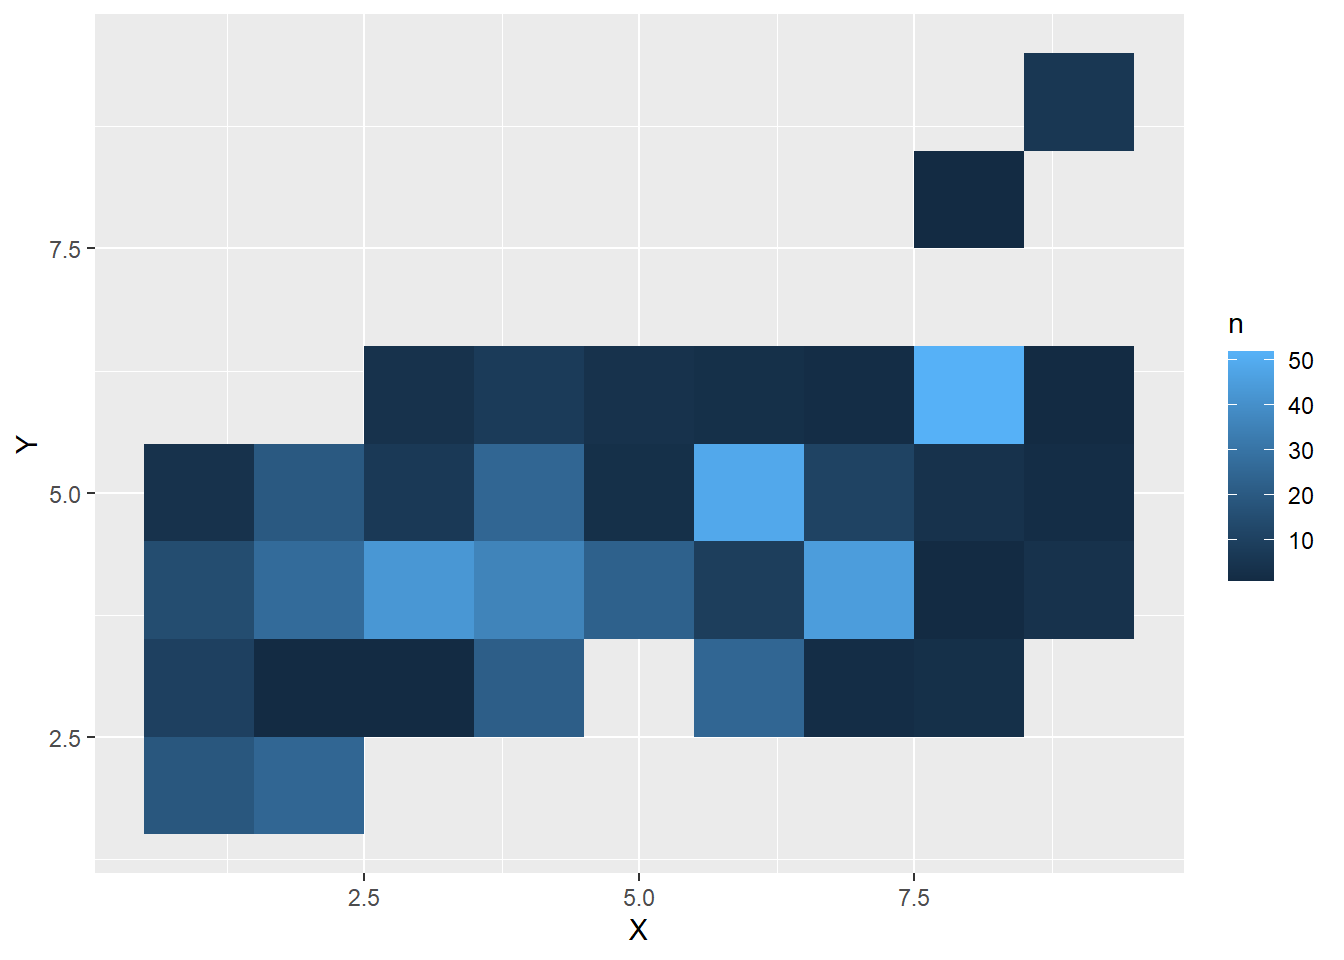
\includegraphics{bookdown-demo_files/figure-latex/unnamed-chunk-76-1.pdf}

  \begin{itemize}
  \tightlist
  \item
    Dodajte stolpec, ki bo za vsak požar izračunal delež požganega območja glede na vse požare na posameznih koordinatah. Za tem smiselno filtrirajte podatke (ali smo v novem stolpcu dobili kakšne nepričakovane, oziroma neveljavne vrednosti?).
  \end{itemize}

\begin{verbatim}
## # A tibble: 509 x 5
##        X     Y month day   area_by_coord
##    <dbl> <dbl> <chr> <chr>         <dbl>
##  1     7     5 mar   fri               0
##  2     7     4 oct   tue               0
##  3     7     4 oct   sat               0
##  4     8     6 mar   fri               0
##  5     8     6 mar   sun               0
##  6     8     6 aug   sun               0
##  7     8     6 aug   mon               0
##  8     8     6 aug   mon               0
##  9     8     6 sep   tue               0
## 10     7     5 sep   sat               0
## # ... with 499 more rows
\end{verbatim}

  \begin{itemize}
  \tightlist
  \item
    Preverite, ali ob vročem vremenu in nizki vlažnosti pogori večji delež območja, ki smo ga izračunali v prejšnji točki, tako da izberete vrstice, kjer je temperatura višja od 0.8 kvantila temperature in vlažnost nižja od 0.2 kvantila vlažnosti ter izračunate povprečje. \(q\)-ti kvantil je ocena števila, za katerega velja, da je \(q\) vrednosti manjših od tega števila. Za računanje kvantilov uporabite funkcijo \texttt{quantile()}. Za primerjavo izračunajte še povprečje te spremenljivke za vse preostale vrstice. Ali se rezultati skladajo z vašo intuicijo?
  \end{itemize}

\begin{verbatim}
## # A tibble: 1 x 1
##   mean_area_by_coord
##                <dbl>
## 1              0.153
\end{verbatim}

\begin{verbatim}
## # A tibble: 1 x 1
##   mean_area_by_coord
##                <dbl>
## 1             0.0555
\end{verbatim}

  \begin{itemize}
  \tightlist
  \item
    Izračunajte povprečje standardiziranih indeksov in ga vstavite kot stolpec pred prvo spremenljivko, ki predstavlja indeks.
  \end{itemize}

\begin{verbatim}
## # A tibble: 509 x 15
## # Rowwise: 
##        X     Y month day   mean_indices FFMC_index DMC_index DC_index ISI_index
##    <dbl> <dbl> <chr> <chr>        <dbl>      <dbl>     <dbl>    <dbl>     <dbl>
##  1     7     5 mar   fri        -1.21     -0.796      -1.32    -1.86   -0.859  
##  2     7     4 oct   tue        -0.304    -0.00502    -1.18     0.480  -0.510  
##  3     7     4 oct   sat        -0.254    -0.00502    -1.05     0.552  -0.510  
##  4     8     6 mar   fri        -0.739     0.193      -1.21    -1.92   -0.00890
##  5     8     6 mar   sun        -0.719    -0.239      -0.934   -1.82    0.122  
##  6     8     6 aug   sun         0.218     0.301      -0.405   -0.256   1.23   
##  7     8     6 aug   mon        -0.0979    0.301      -0.349   -0.225  -0.118  
##  8     8     6 aug   mon         0.320     0.157       0.530    0.232   0.361  
##  9     8     6 sep   tue         0.120     0.0669      0.283    0.575  -0.445  
## 10     7     5 sep   sat         0.0375    0.337      -0.363    0.599  -0.423  
## # ... with 499 more rows, and 6 more variables: temp <dbl>, RH <dbl>,
## #   wind <dbl>, rain <dbl>, area <dbl>, area_by_coord <dbl>
\end{verbatim}
\end{enumerate}

  \bibliography{book.bib,packages.bib}

\end{document}
